\documentclass[a4paper]{article}

%% Language and font encodings
\usepackage[french]{babel}
\usepackage[utf8x]{inputenc}
\usepackage[T1]{fontenc}

%% Sets page size and margins
\usepackage[a4paper,top=3cm,bottom=3cm,left=2cm,right=2cm,marginparwidth=2cm]{geometry}

%% Useful packages
\usepackage{amsmath}
\usepackage{graphicx}
\usepackage[colorinlistoftodos]{todonotes}
\usepackage[colorlinks=true, allcolors=black]{hyperref}
\usepackage{fourier-orns}
\usepackage{titlesec}
\usepackage{fancyhdr}
\usepackage{fancyvrb}
\usepackage{float}
\pagestyle{fancy} 
\setcounter{tocdepth}{5}


%% Tikz stuff
\usepackage{tikz}
\usetikzlibrary{calc, arrows}
\tikzstyle{incolore} = [rectangle, rounded corners, draw=black, minimum height=1cm, minimum width=3cm, text width=3cm, text centered]



\usepackage{libertine}
\newcommand{\hsp}{\hspace{20pt}}
\newcommand{\HRule}{\rule{\linewidth}{0.5mm}}





\renewcommand{\headrulewidth}{1pt}
\fancyhead[C]{} 
\fancyhead[L]{}
\fancyhead[R]{\footnotesize{\leftmark}}

\renewcommand{\footrulewidth}{1pt}
\fancyfoot[C]{} 
\fancyhead[L]{}
\fancyfoot[R]{\thepage}

\definecolor{Zgris}{rgb}{0.87,0.85,0.85}

\usepackage{eso-pic,graphicx}
\usepackage{xcolor}
\newcommand{\bgimg}[1]{
\AddToShipoutPicture
   {
      \put(\LenToUnit{0 cm},\LenToUnit{0 cm})
      {
            \includegraphics[width=\paperwidth,height=\paperheight]{#1} 
      }
   }
}
\begin{document}




%%\bgimg{Image_15.jpg}

















\begin{titlepage}
    \begin{sffamily}
        \begin{center}
            
\includegraphics[width=5cm]{images/LogoHenallux.PNG}~\\[1.5cm]
            \textsc{\Large Rapport de laboratoire}\\[1.5cm]

            % Title
            \HRule \\[0.4cm]
            { \huge \bfseries Sixième laboratoire : représentation des signaux – analyse de Fourier \\[0.4cm] }
            \HRule \\[2cm]

            % Author and supervisor
            \begin{minipage}{0.4\textwidth}
                \begin{flushleft} \large
                    Roumache Grégoire\\
                    Sénéchal Julien\\
                    Robert Alexandre\\
                    Wallemme Maxime\\
                    Kenmeugne Lionel\\
                    Didion Charles
                \end{flushleft}
            \end{minipage}
            \begin{minipage}{0.55\textwidth}
                \begin{flushright} \large
                    Laboratoire de sciences appliquées à l'informatique\\
                    Sécurité des systèmes, technologie de l'informatique\\
                    Hénallux\\
                    Première année, groupe H \\
                    Année académique 2019-2020\\
                \end{flushright}
            \end{minipage}
            \vfill

            % Bottom of the page
            {\large 2 Avril 2020}
        \end{center}
    \end{sffamily}
\end{titlepage}







\let\cleardoublepage\clearpage















\section{Introduction}





Pour ce laboratoire de Sciences Appliquées à l'informatique, nous voyons la représentation des signaux et l'analyse de Fourier. Nous commençons ce rapport avec un rappel théorique sur les représentations spectrale et temporelle qui aident à la compréhension de la manipulation pratique où nous verrons quatres types de signaux. Ces différents types de signaux sont les signaux carré, en dent de scie, un \textit{autre signal} et un signal personnel que nous avons pu choisir nous même. Pour ce signal personnel, nous avons choisi un signal triangulaire.















\section{Rappels théoriques}










\subsection{Représentation spectrale et représentation temporelle}





La représentation temporelle d'un signal sonore monte l'évolution de l'intensité du son en fonction du temps. La représentation spectrale d'un son montre la variation de l'intensité du son en fonction de la fréquence sonore. Ces deux types de représentations sont très utilisées dans la partie pratique de ce rapport.










\subsection{Séries de Fourier}





Les séries de Fourier sont utiles pour étudier des fonction périodiques en mathématique. La physique ondulaire se sert donc volontier de cet outil. Une série de Fourier est une la somme pondérée d'une suite de sinusoïdes dont les fréquences sont liées. Cette somme approxime une fonction périodique donnée.













\section{Manipulation pratique}










\subsection{Signal carré}





La série de Fourier d'un signal carré est donné par la série suivante, qui vient de l'énoncé de la manipulation:
\[ x(t) = \frac{4E}{\pi} \bigg( \sin \omega t + \frac{\sin 3 \omega t}{3} + \frac{\sin 5 \omega t}{5} + ... \bigg) \]
Les quatres premiers signaux que nous devons générer sont donc:
\begin{enumerate}
    \item signal = $\displaystyle \frac{4E}{\pi} \sin \omega t $, amplitude = 0,637, fréquence = 300 Hz
    \item signal = $\displaystyle \frac{4E}{\pi} \frac{\sin 3 \omega t}{3} $, amplitude = 0,212, fréquence = 900 Hz
    \item signal = $\displaystyle \frac{4E}{\pi} \frac{\sin 5 \omega t}{5} $, amplitude = 0,127, fréquence = 1500 Hz
    \item signal = $\displaystyle \frac{4E}{\pi} \frac{\sin 7 \omega t}{7} $, amplitude = 0,091, fréquence = 2100 Hz
\end{enumerate}
\textbf{Remarque:} E = 0,5 et la fréquence du signal carré est de 300 Hz.





%%%%%%%%%%%%%%%%%%%%%%%%%

Comme il était demandé dans la manipulation, nous avons généré les deux premières sinusoïdes. Elles sont représentées sur les figures \ref{fig:SignalCarre005} et \ref{fig:SignalCarre009}. Leurs représentation spectrales sont illustrées par les figures \ref{fig:SignalCarre021} et \ref{fig:SignalCarre022}.

%%%%%%%%%%%%%%%%%%%%%%%%%

\begin{figure}[H]
    \centering
    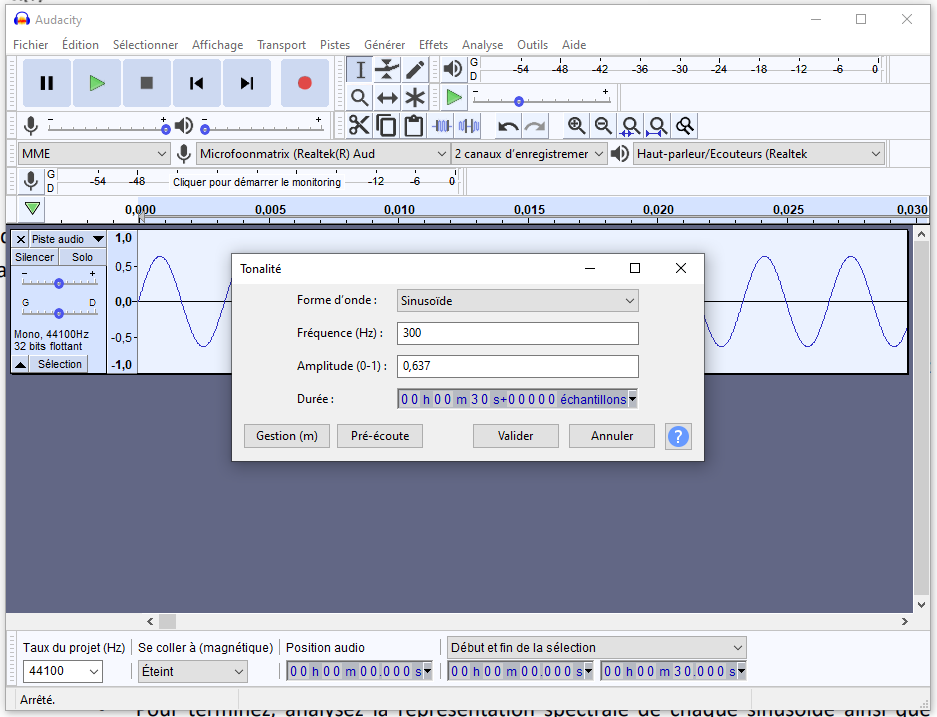
\includegraphics[width=0.85\textwidth]{images/SignalCarre005.PNG}
    \caption{Première sinusoïde du signal carré}
    \label{fig:SignalCarre005}
\end{figure}

\begin{figure}[H]
    \centering
    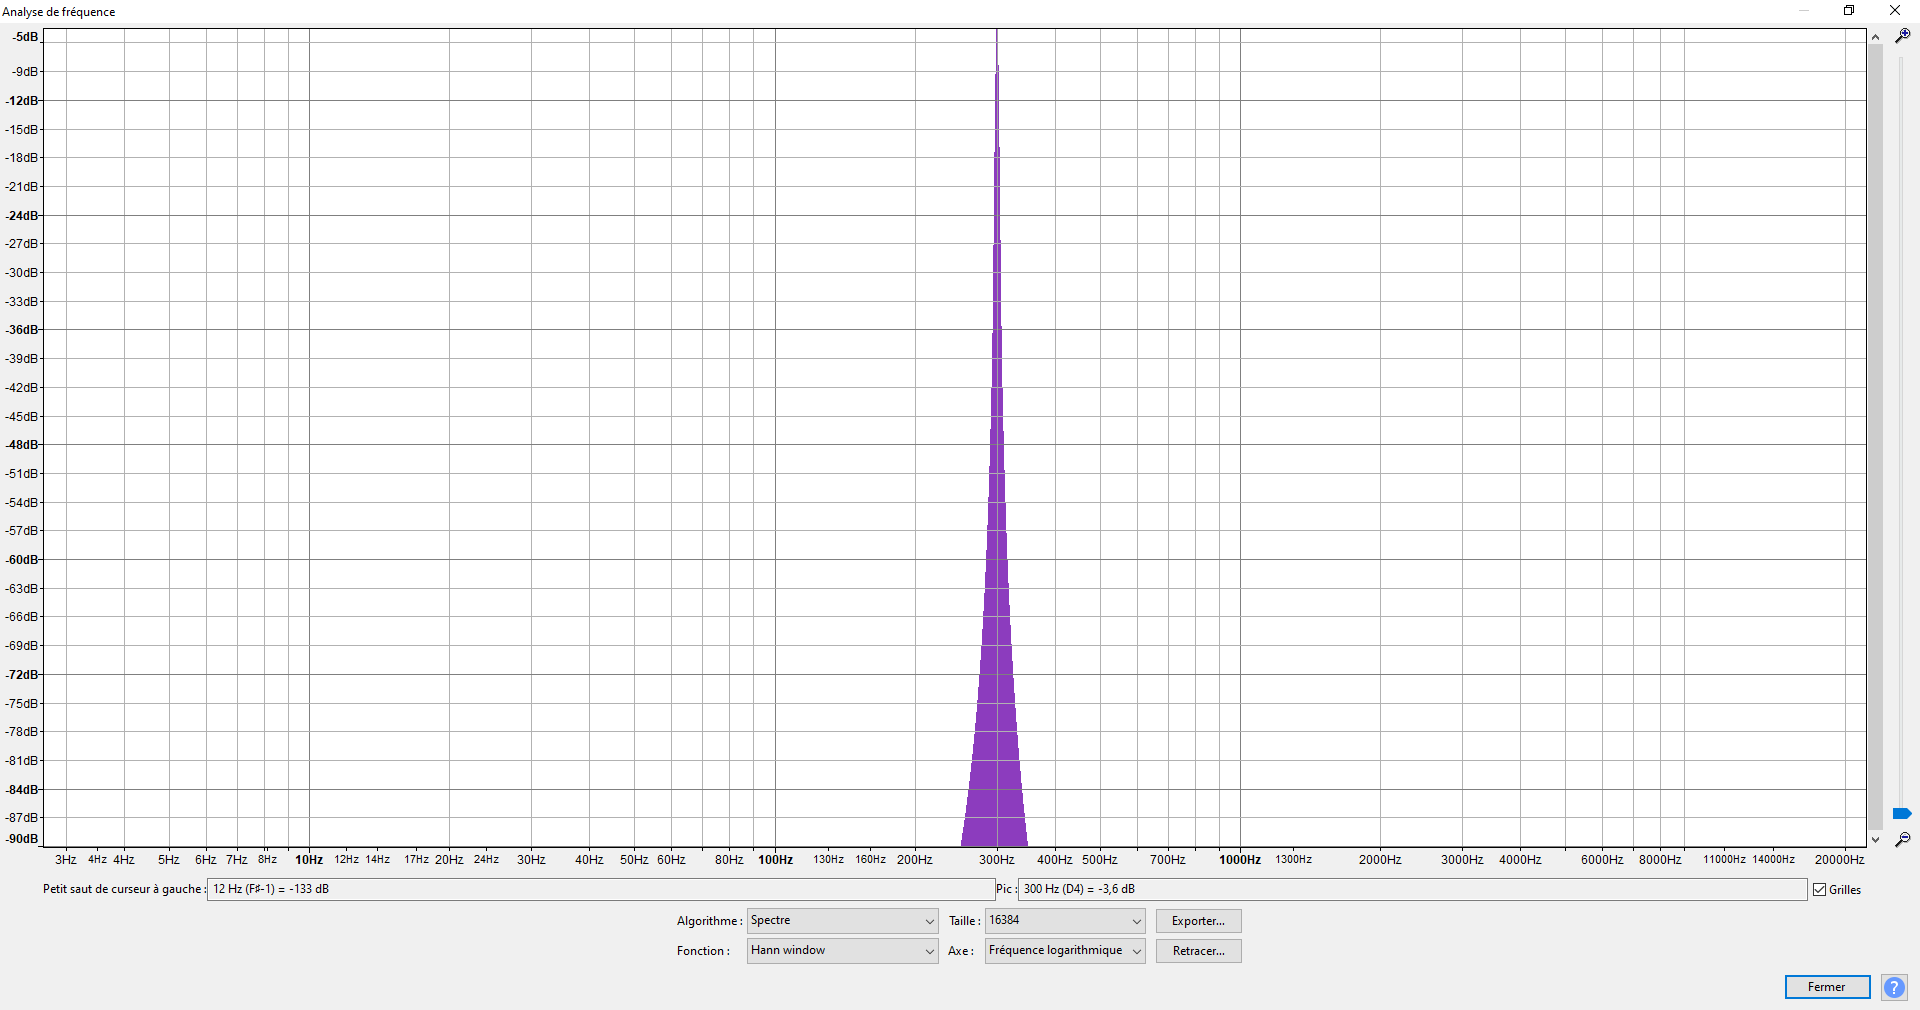
\includegraphics[width=0.85\textwidth]{images/SignalCarre021.PNG}
    \caption{Représentation spectrale de la première sinusoïde du signal carré}
    \label{fig:SignalCarre021}
\end{figure}

%%%%%%%%%%%%%%%%%%%%%%%%%

\begin{figure}[H]
    \centering
    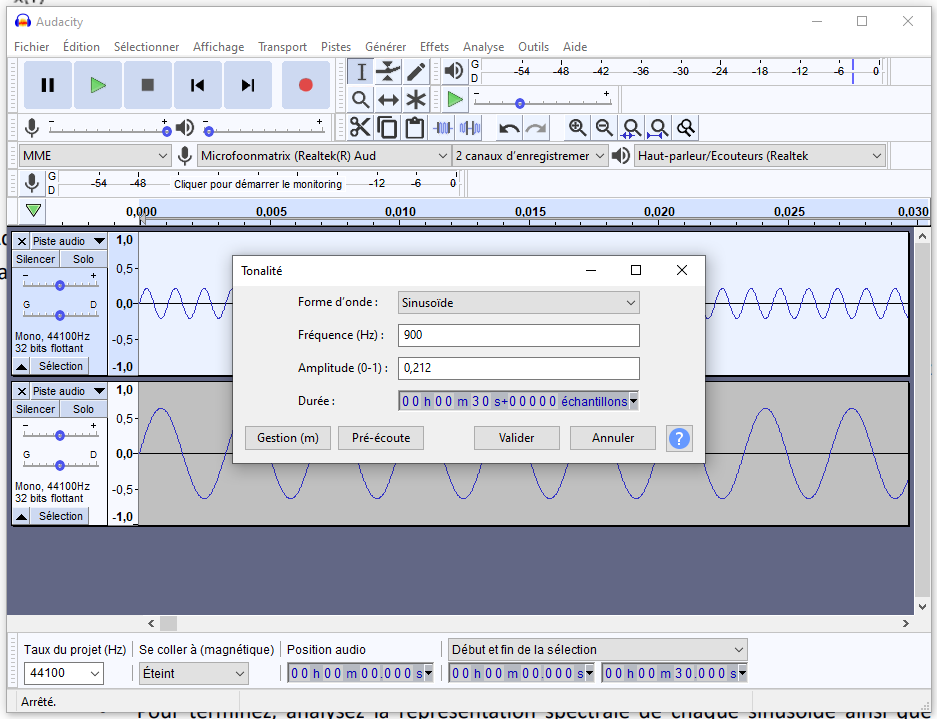
\includegraphics[width=0.85\textwidth]{images/SignalCarre009.PNG}
    \caption{Ajout de la deuxième sinusoïde du signal carré}
    \label{fig:SignalCarre009}
\end{figure}

\begin{figure}[H]
    \centering
    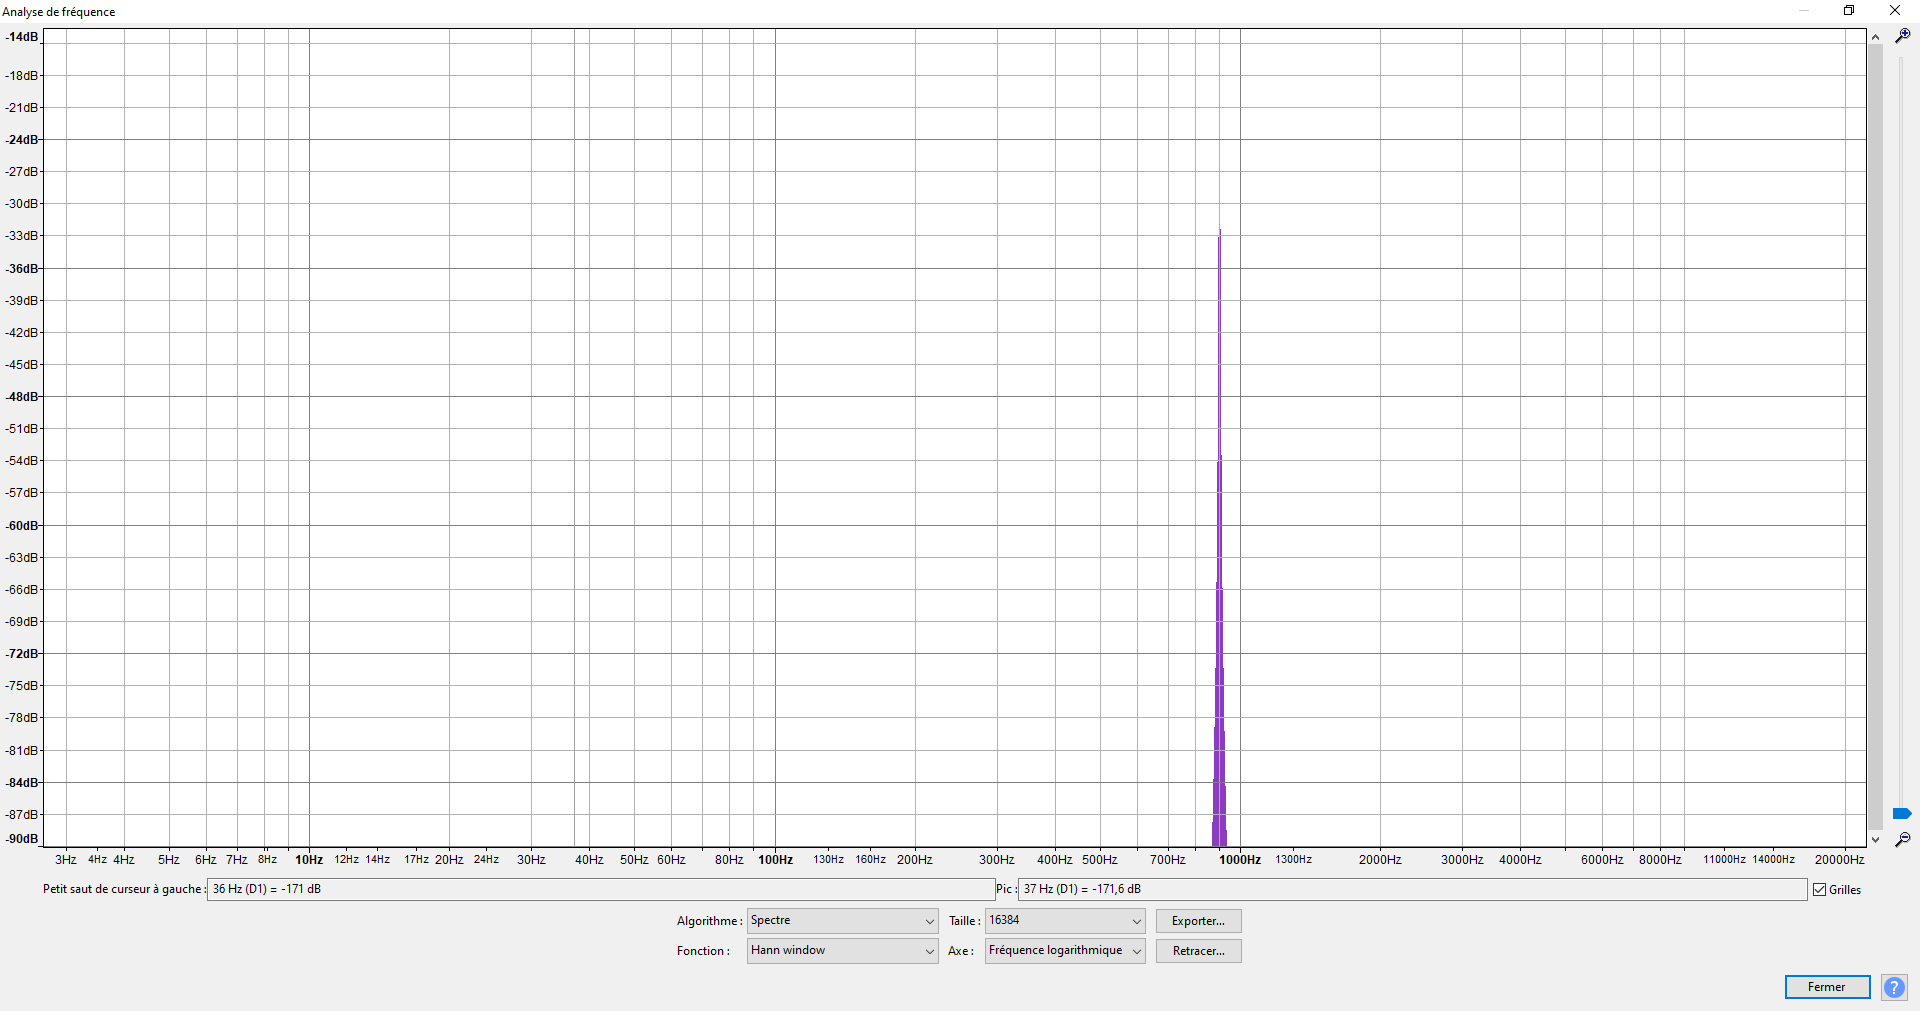
\includegraphics[width=0.85\textwidth]{images/SignalCarre022.PNG}
    \caption{Représentation spectrale de la deuxième sinusoïde du signal carré}
    \label{fig:SignalCarre022}
\end{figure}

%%%%%%%%%%%%%%%%%%%%%%%%%

Une fois que les deux premières sinusoïdes ont été générées, nous avons utiliser la fonction de mixage pour en générer une nouvelle comme il était demandé dans l'énoncé et l'onde qui en résulte est illustrée par la figure \ref{fig:SignalCarre010} et sa représentation spectrale par la figure \ref{fig:SignalCarre011}.

%%%%%%%%%%%%%%%%%%%%%%%%%

\begin{figure}[H]
    \centering
    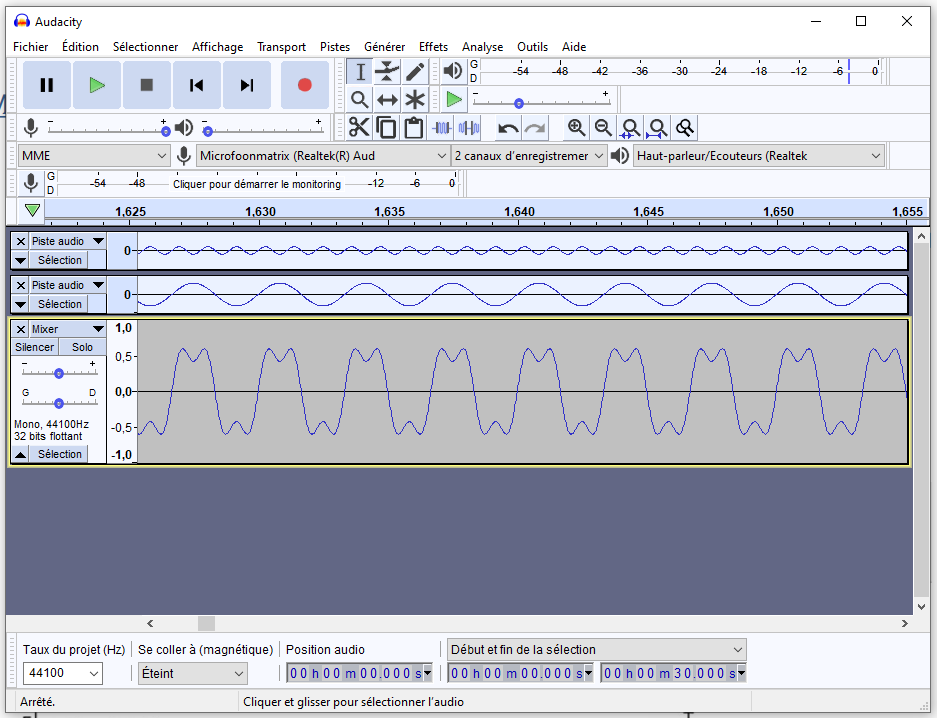
\includegraphics[width=0.85\textwidth]{images/SignalCarre010.PNG}
    \caption{Génération et visualisation du signal approximant le signal carré (2 sinusoïdes)}
    \label{fig:SignalCarre010}
\end{figure}

\begin{figure}[H]
    \centering
    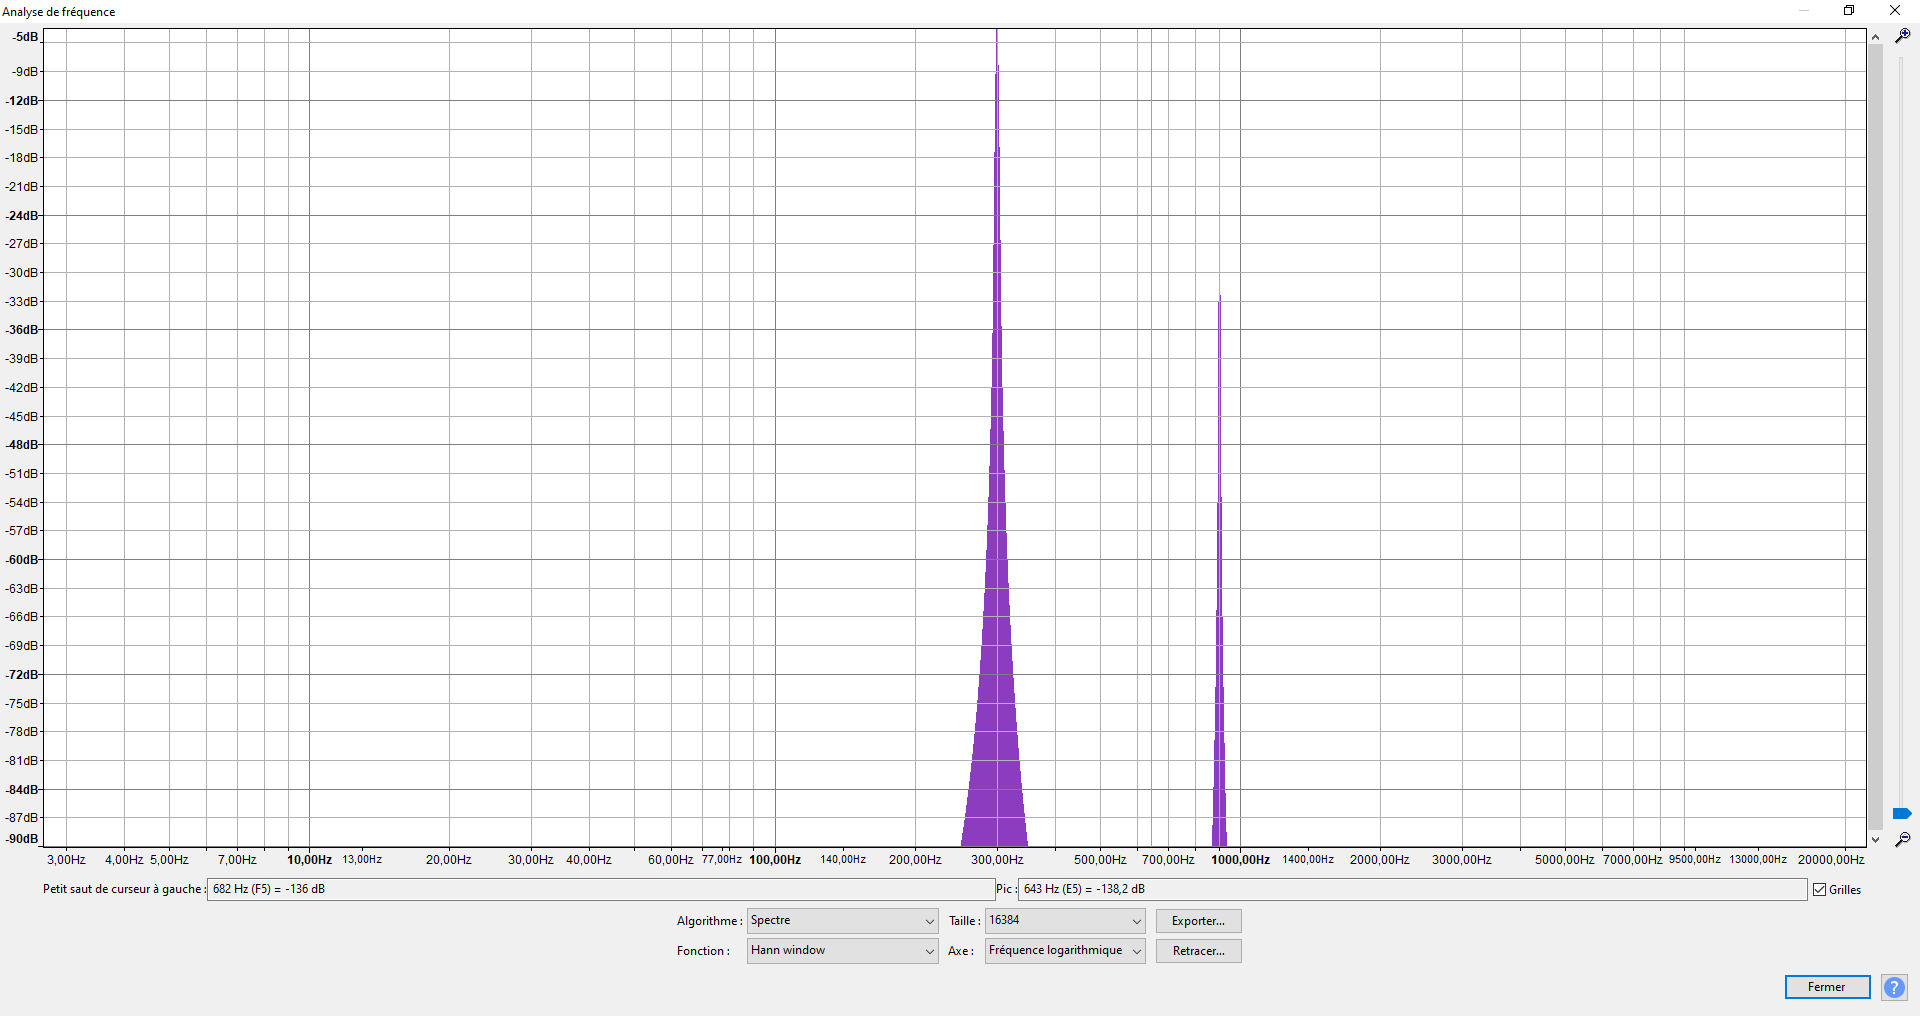
\includegraphics[width=0.85\textwidth]{images/SignalCarre011.PNG}
    \caption{Représentation spectrale du signal approximant le signal carré (2 sinusoïdes)}
    \label{fig:SignalCarre011}
\end{figure}

%%%%%%%%%%%%%%%%%%%%%%%%%

Puisque nous avions généré l'approximation du signal carré avec deux sinusoïdes, il ne nous restait qu'à ajouter les deux suivantes et générer une nouvelle approximation du signal carré avec quatre sinusoïdes. Cette nouvelle approximation est représentée par la figure \ref{fig:SignalCarre019} et sa représentation spectrale est donnée par la figure \ref{fig:SignalCarre020}.

%%%%%%%%%%%%%%%%%%%%%%%%%

\begin{figure}[H]
    \centering
    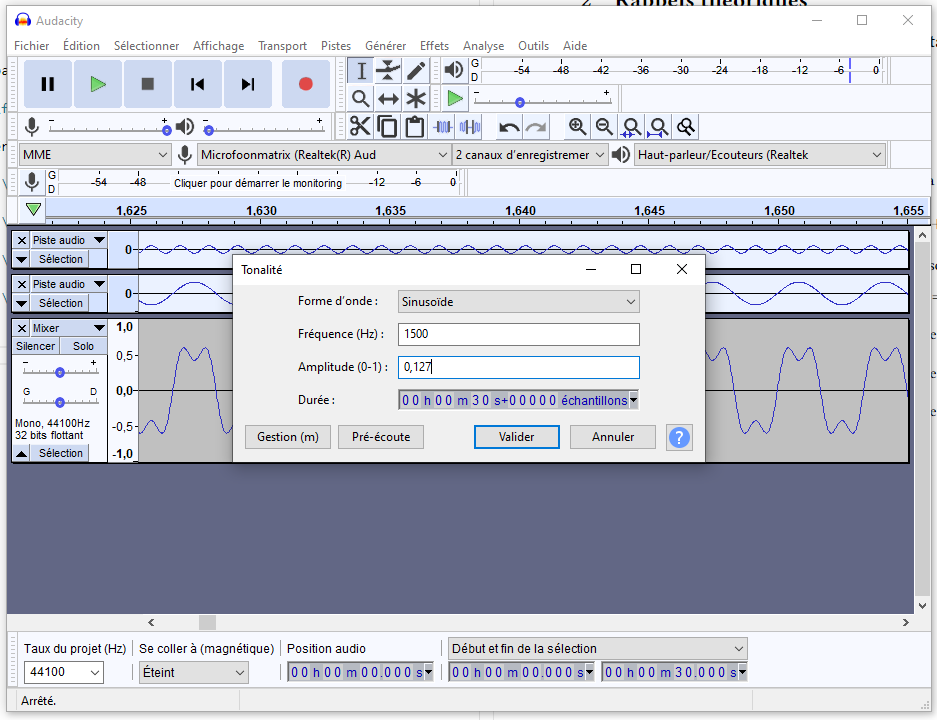
\includegraphics[width=0.85\textwidth]{images/SignalCarre012.PNG}
    \caption{Ajout de la troisième sinusoïde du signal carré}
    \label{fig:SignalCarre012}
\end{figure}

\begin{figure}[H]
    \centering
    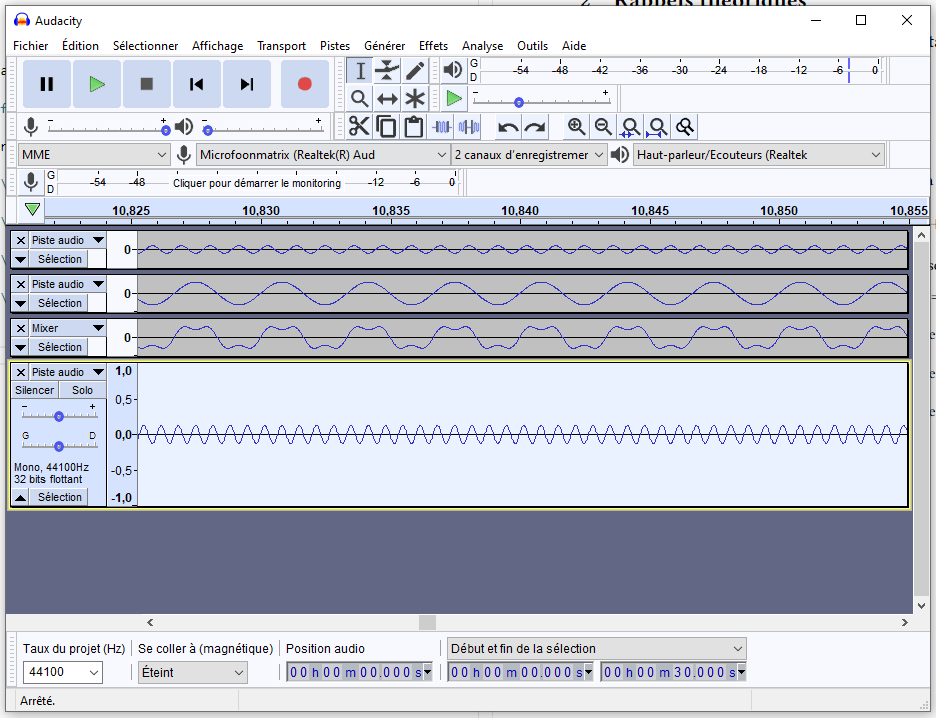
\includegraphics[width=0.85\textwidth]{images/SignalCarre013.PNG}
    \caption{Visualisation de la troisième sinusoïde du signal carré}
    \label{fig:SignalCarre013}
\end{figure}

\begin{figure}[H]
    \centering
    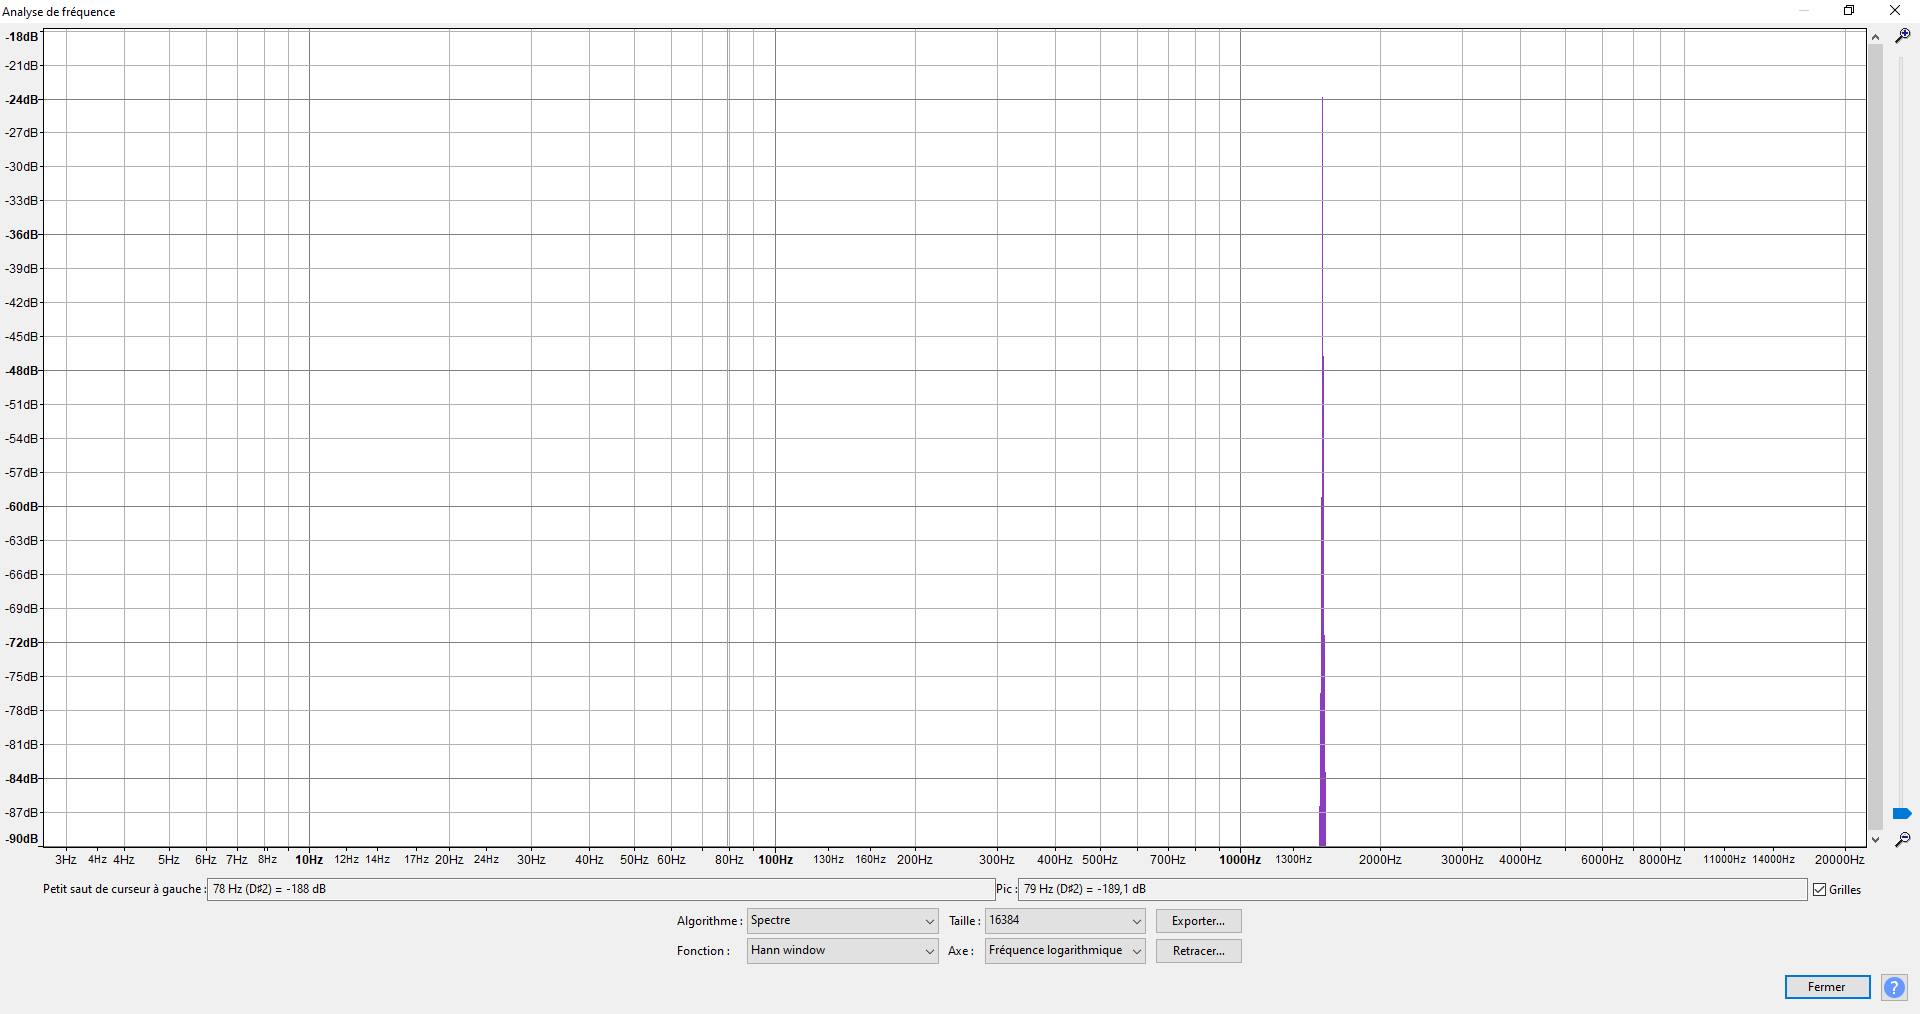
\includegraphics[width=0.85\textwidth]{images/SignalCarre023.PNG}
    \caption{Représentation spectrale de la troisième sinusoïde du signal carré}
    \label{fig:SignalCarre023}
\end{figure}

%%%%%%%%%%%%%%%%%%%%%%%%%

\begin{figure}[H]
    \centering
    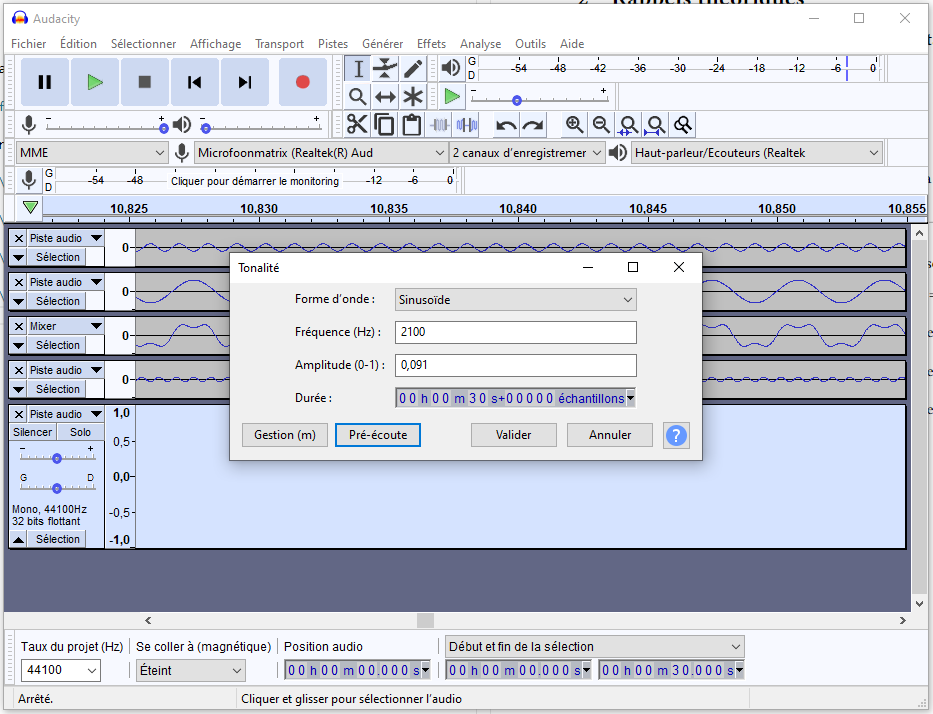
\includegraphics[width=0.85\textwidth]{images/SignalCarre015.PNG}
    \caption{Ajout de la quatrième sinusoïde du signal carré}
    \label{fig:SignalCarre015}
\end{figure}

\begin{figure}[H]
    \centering
    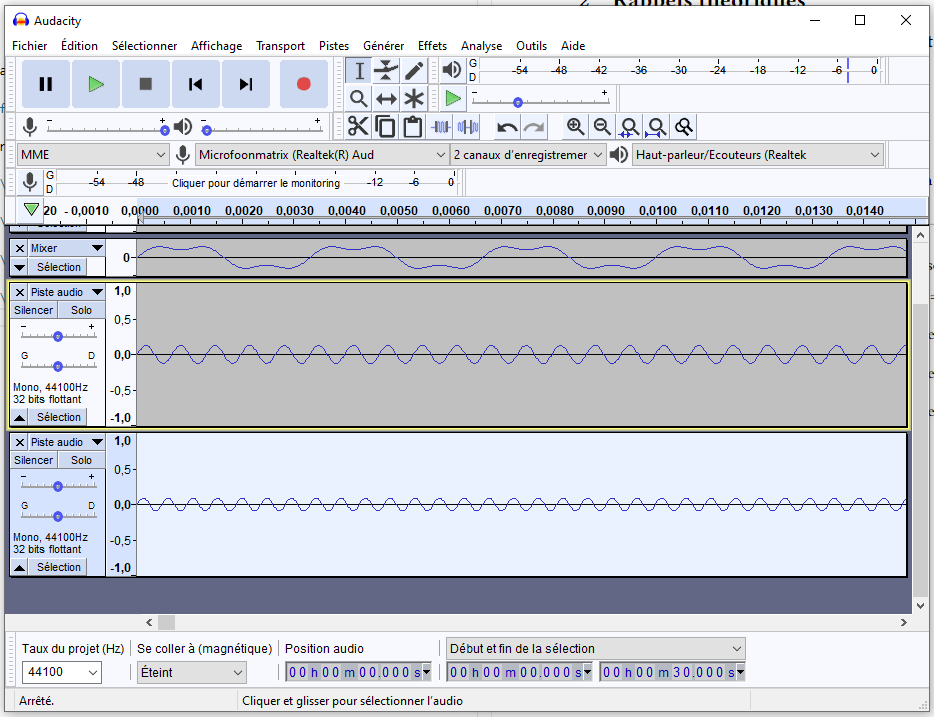
\includegraphics[width=0.85\textwidth]{images/SignalCarre016.PNG}
    \caption{Visualisation de la quatrième sinusoïde du signal carré}
    \label{fig:SignalCarre016}
\end{figure}

\begin{figure}[H]
    \centering
    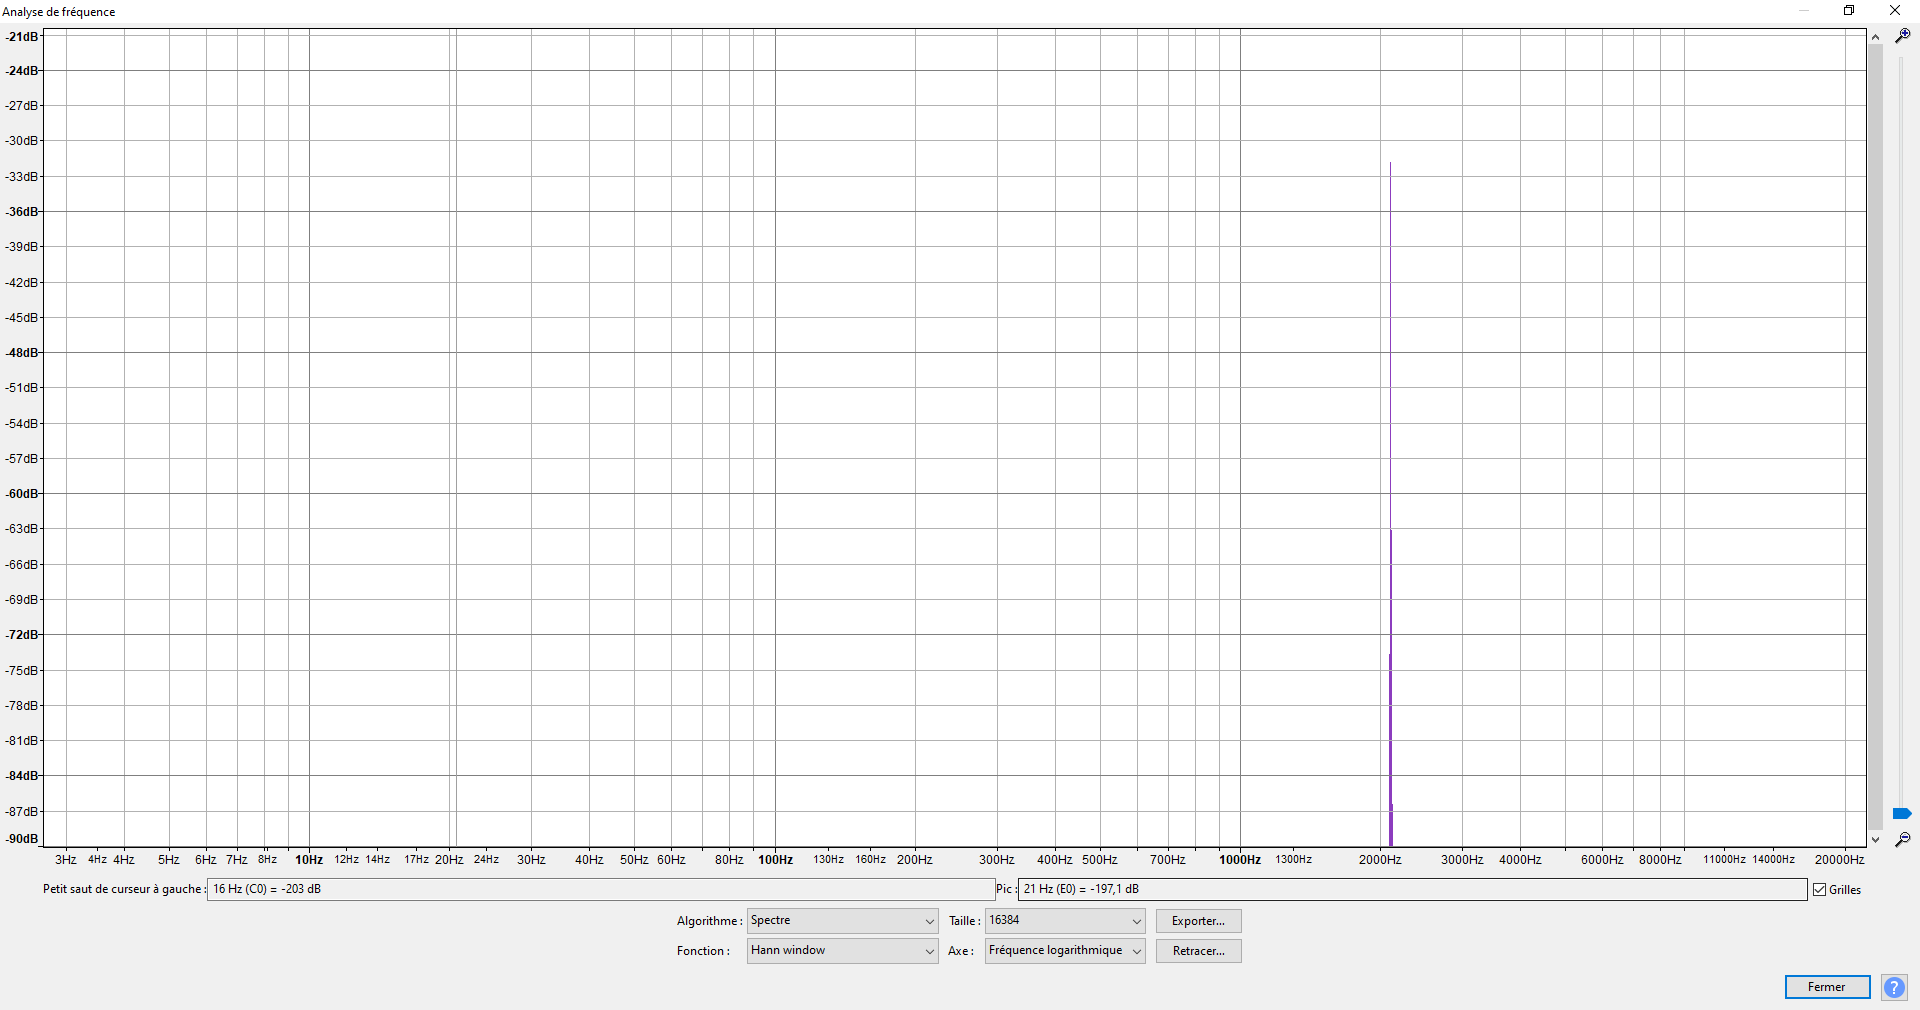
\includegraphics[width=0.85\textwidth]{images/SignalCarre024.PNG}
    \caption{Représentation spectrale de la quatrième sinusoïde du signal carré}
    \label{fig:SignalCarre024}
\end{figure}

%%%%%%%%%%%%%%%%%%%%%%%%%

\begin{figure}[H]
    \centering
    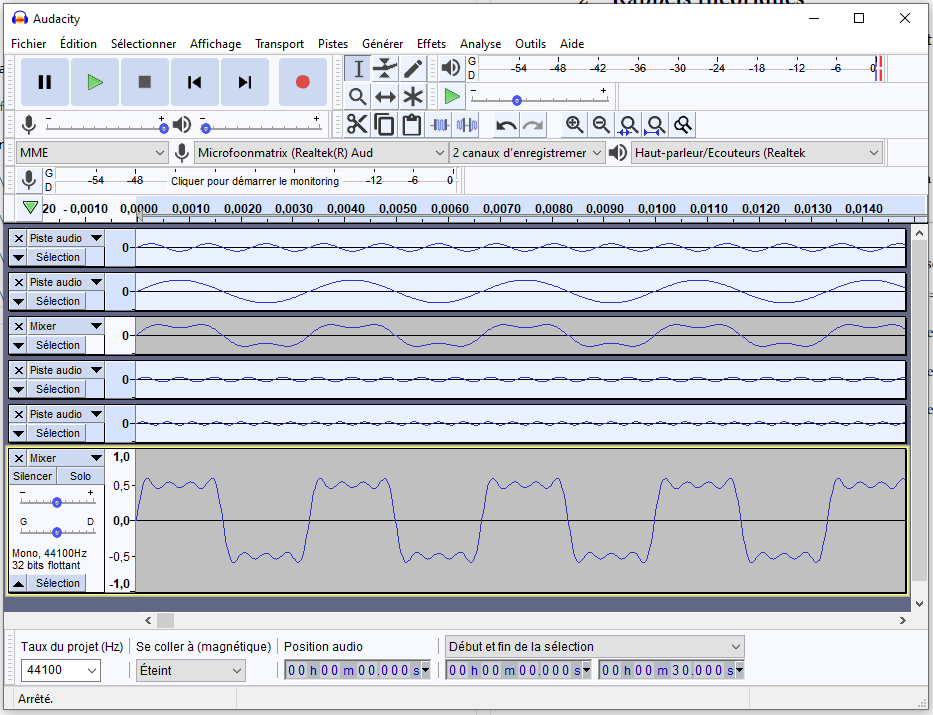
\includegraphics[width=0.85\textwidth]{images/SignalCarre019.PNG}
    \caption{Génération et visualisation du signal approximant le signal carré}
    \label{fig:SignalCarre019}
\end{figure}

\begin{figure}[H]
    \centering
    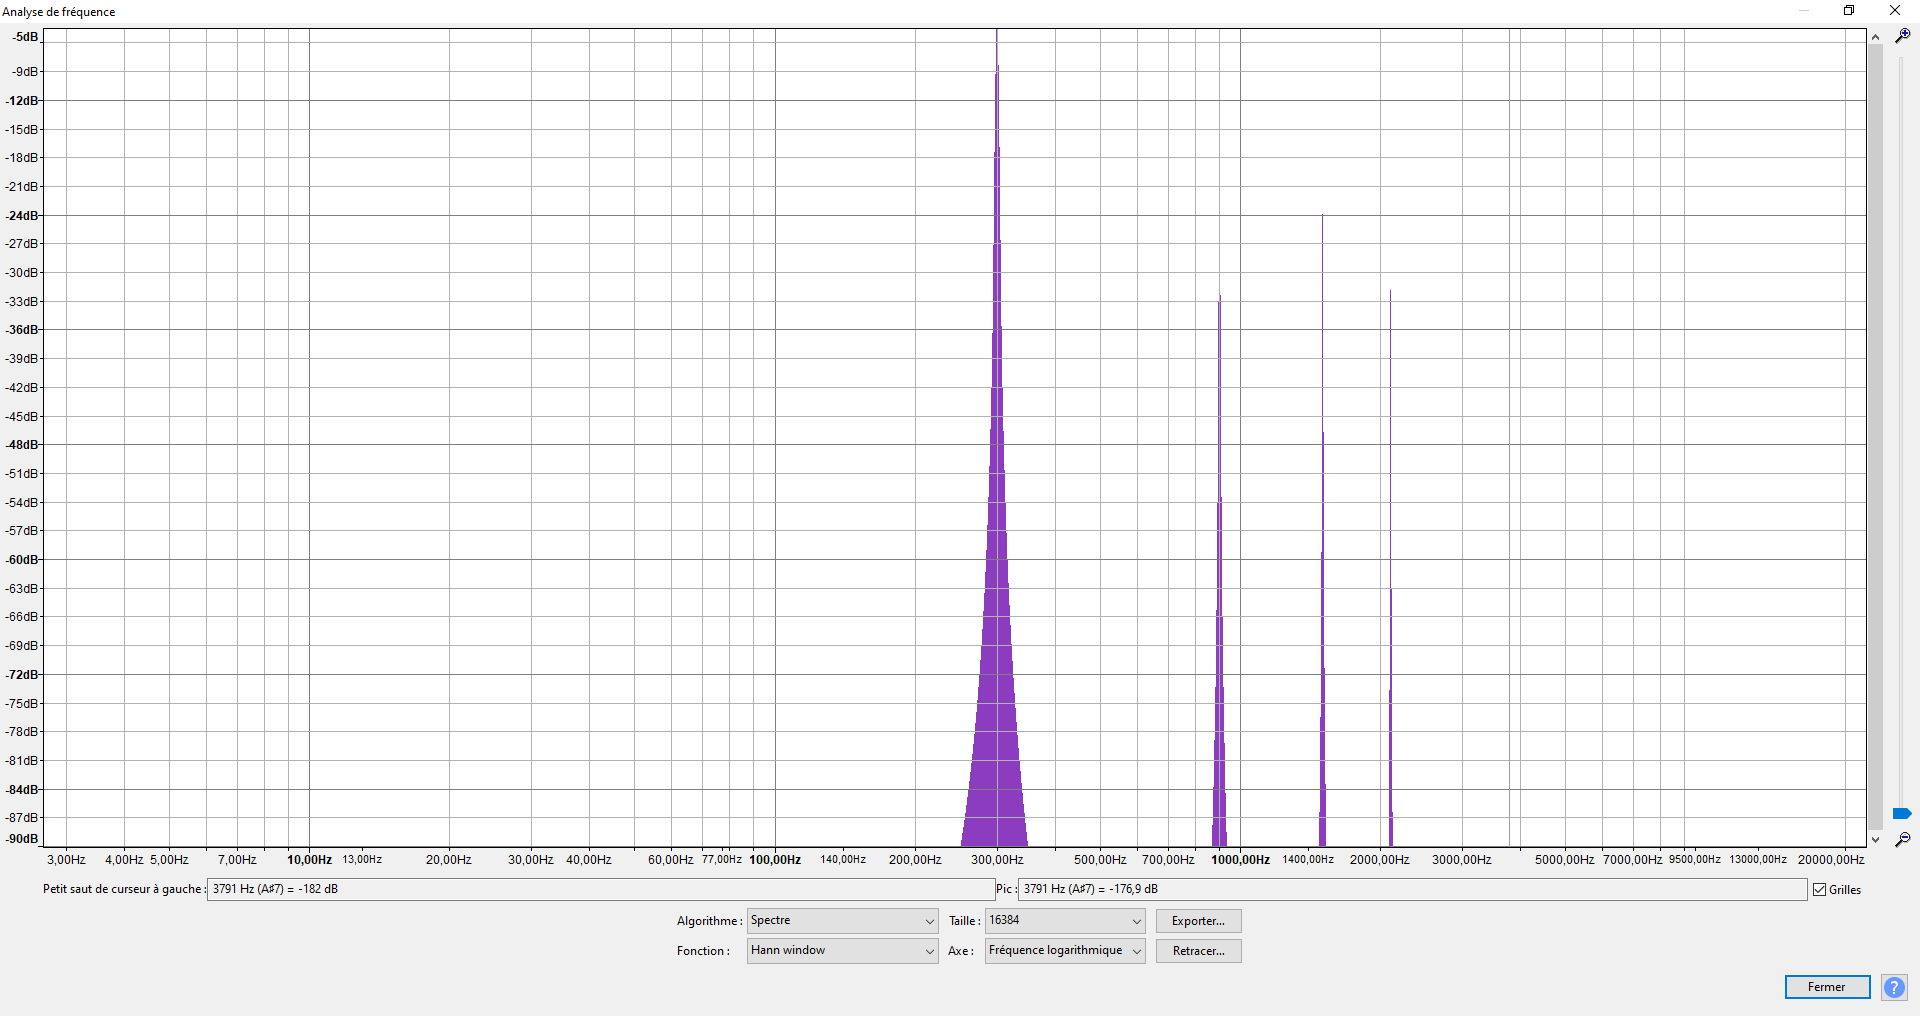
\includegraphics[width=0.85\textwidth]{images/SignalCarre020.PNG}
    \caption{Représentation spectrale du signal approximant le signal carré}
    \label{fig:SignalCarre020}
\end{figure}

%%%%%%%%%%%%%%%%%%%%%%%%%

Désormais, il ne nous restait plus qu'à comparer avec un "vrai" signal carré généré par le logiciel Audacity directement. C'est ce que nous avons fait sur la figure \ref{fig:SignalCarre001}. Le résultat, c'est à dire la représentation temporelle de l'onde est sur la figure \ref{fig:SignalCarre002} et la représentation spectrale de ce signal carré est sur la figure \ref{fig:SignalCarre003}. Enfin, nous avons mis en évidence le fréquences des sinusoïdes que nous avons utilisé dans l'approximation du signal carré sur la représentation spectrale du vrai signal carré généré par Audacity sur la figure \ref{fig:SignalCarre004}.

%%%%%%%%%%%%%%%%%%%%%%%%%

\begin{figure}[H]
    \centering
    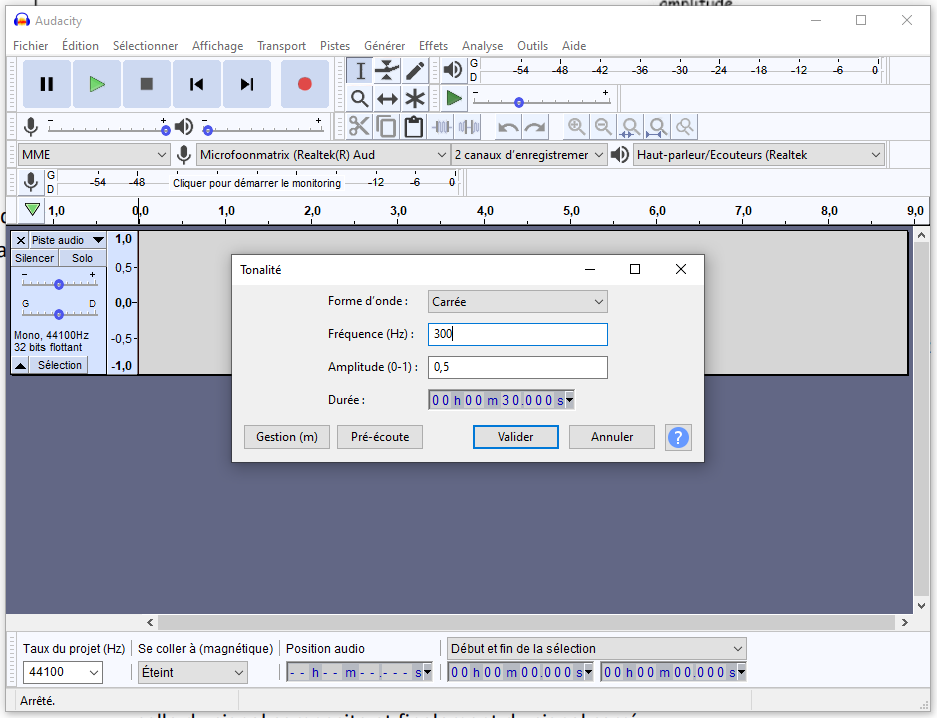
\includegraphics[width=0.85\textwidth]{images/SignalCarre001.PNG}
    \caption{Génération du signal carré}
    \label{fig:SignalCarre001}
\end{figure}

\begin{figure}[H]
    \centering
    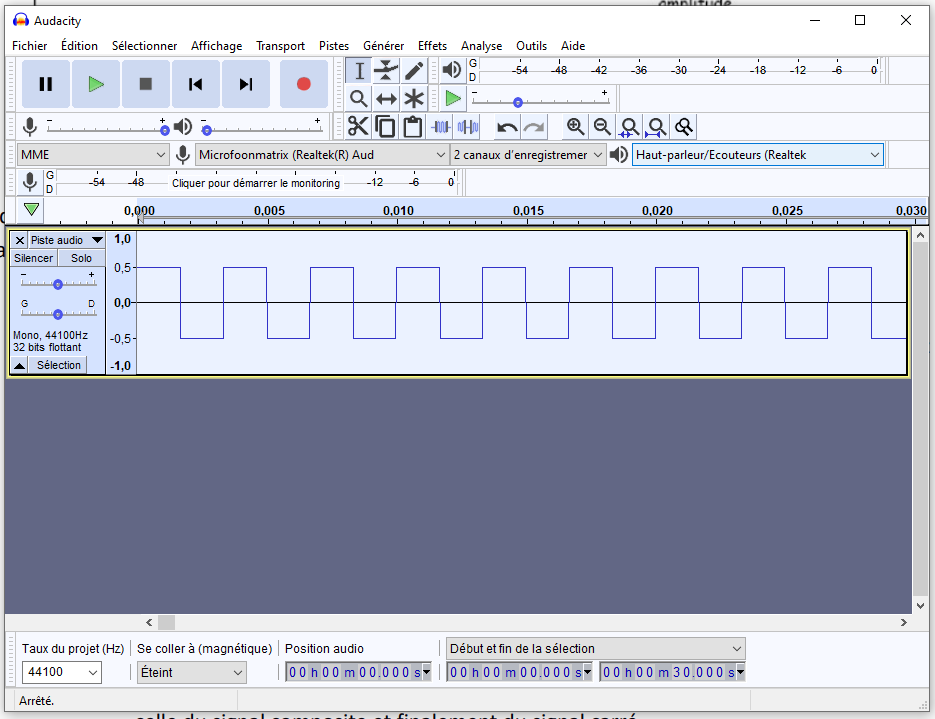
\includegraphics[width=0.85\textwidth]{images/SignalCarre002.PNG}
    \caption{Visualisation du signal carré}
    \label{fig:SignalCarre002}
\end{figure}

\begin{figure}[H]
    \centering
    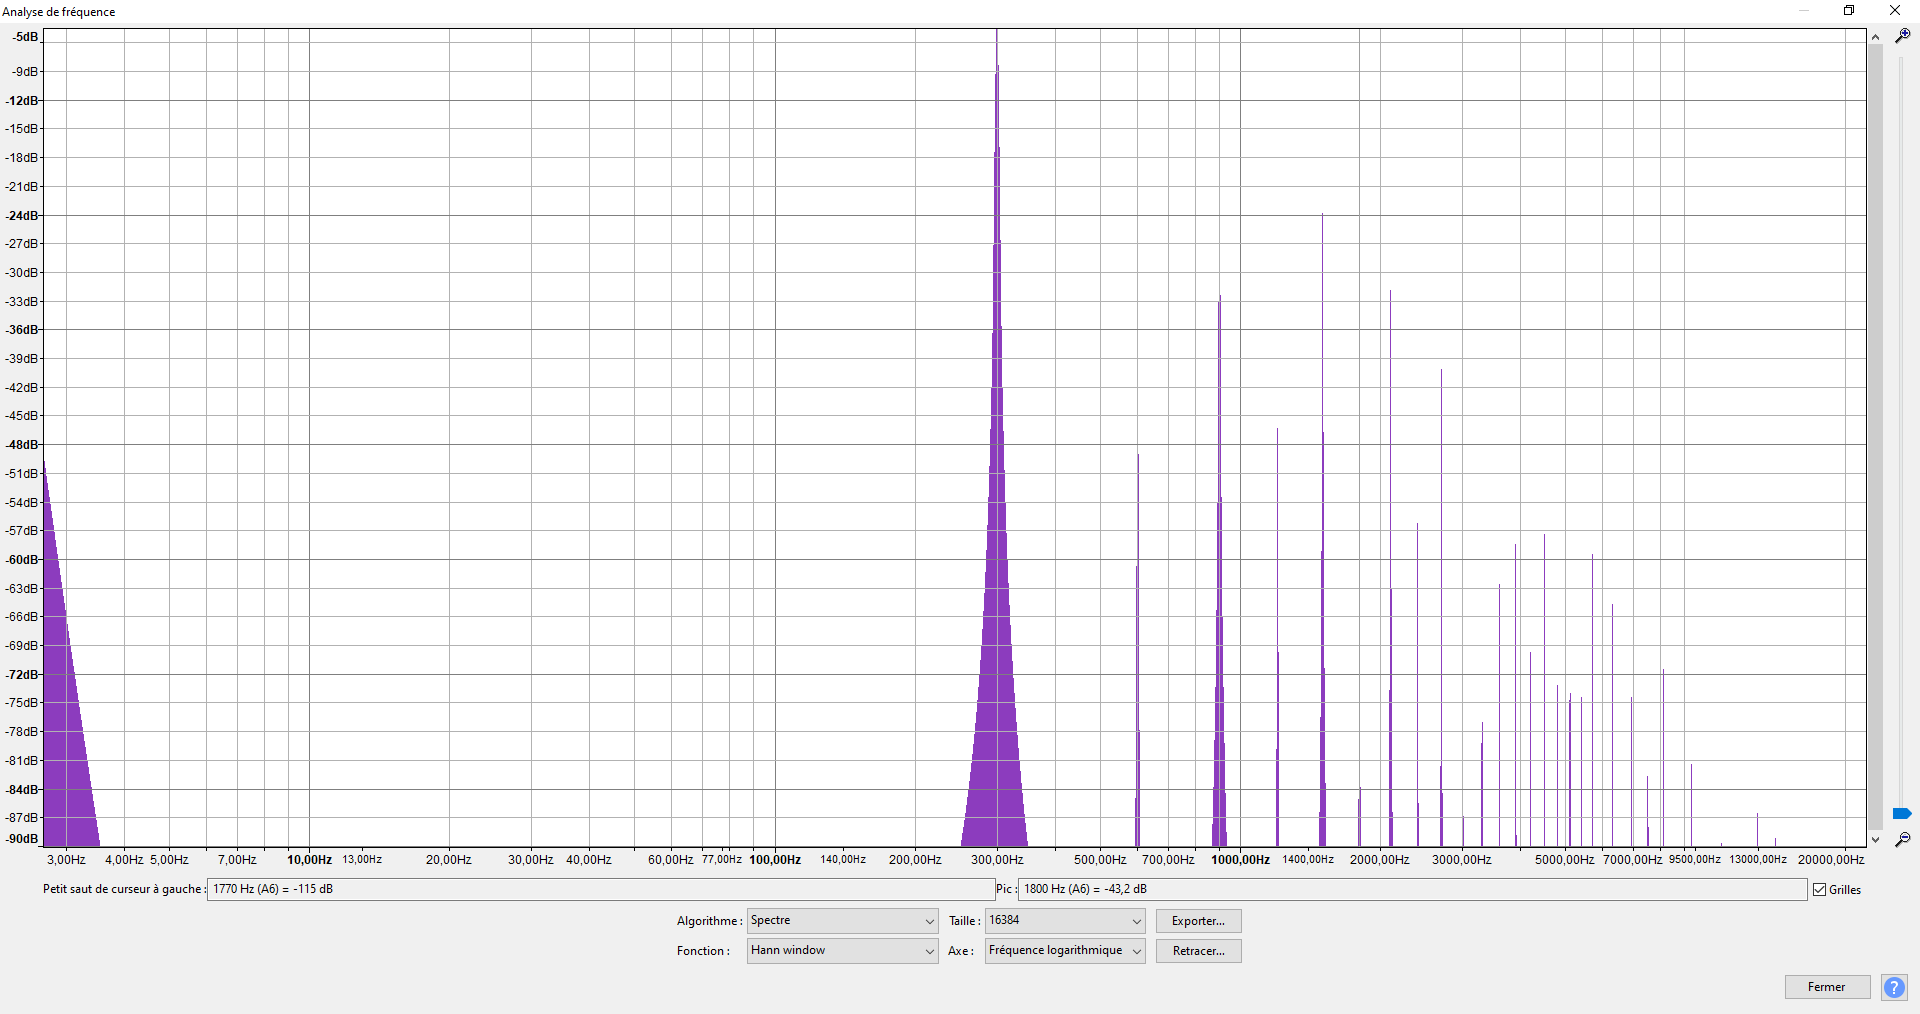
\includegraphics[width=0.85\textwidth]{images/SignalCarre003.PNG}
    \caption{Représentation spectrale du signal carré}
    \label{fig:SignalCarre003}
\end{figure}

\begin{figure}[H]
    \centering
    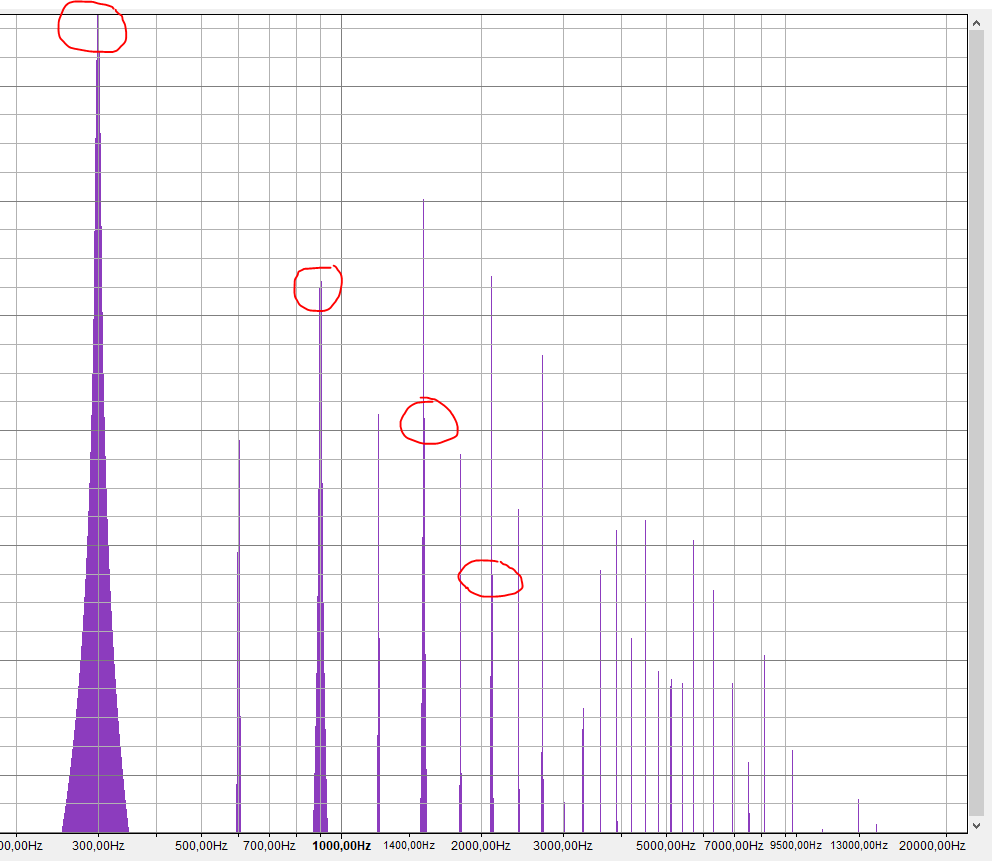
\includegraphics[width=0.85\textwidth]{images/SignalCarre004.PNG}
    \caption{Mise en évidence des fréquences des sinusoïdes sur la représentation spectrale du signal carré}
    \label{fig:SignalCarre004}
\end{figure}

%%%%%%%%%%%%%%%%%%%%%%%%%










\subsection{Signal en dent de scie}





La série de Fourier d'un signal en dent de scie est donné par la série suivante, qui vient de l'énoncé de la manipulation:
\[ x(t) = \frac{2E}{\pi} \bigg( \sin \omega t - \frac{\sin 2 \omega t}{2} + \frac{\sin 3 \omega t}{3} - ... \bigg) \]
Les quatres premiers signaux que nous devons générer sont donc:
\begin{enumerate}
    \item signal = $\displaystyle +\frac{2E}{\pi} \sin \omega t $, amplitude = 0,509, fréquence = 500 Hz
    \item signal = $\displaystyle -\frac{2E}{\pi} \frac{\sin 2 \omega t}{2} $, amplitude = 0,255, fréquence = 1000 Hz
    \item signal = $\displaystyle +\frac{2E}{\pi} \frac{\sin 3 \omega t}{3} $, amplitude = 0,170, fréquence = 1500 Hz
    \item signal = $\displaystyle -\frac{2E}{\pi} \frac{\sin 4 \omega t}{4} $, amplitude = 0,127, fréquence = 2000 Hz
\end{enumerate}
\textbf{Remarque:} E = 0,8 et la fréquence du signal en dent de scie est de 500 Hz.





%%%%%%%%%%%%%%%%%%%%%%%%%

Cette fois-ci, l'énoncé de la manipulation ne nous demandait pas de regarder le signal en dent de scie \textit{après} avoir généré son approximation. Commençons donc par regarder ce signal que nous avons créé sur la figure \ref{fig:DentScie001} et dont la représentation temporelle est illustrée par la figure \ref{fig:DentScie002} tandis que sa représentation spectrale est sur la figure \ref{fig:DentScie003}.

%%%%%%%%%%%%%%%%%%%%%%%%%

\begin{figure}[H]
    \centering
    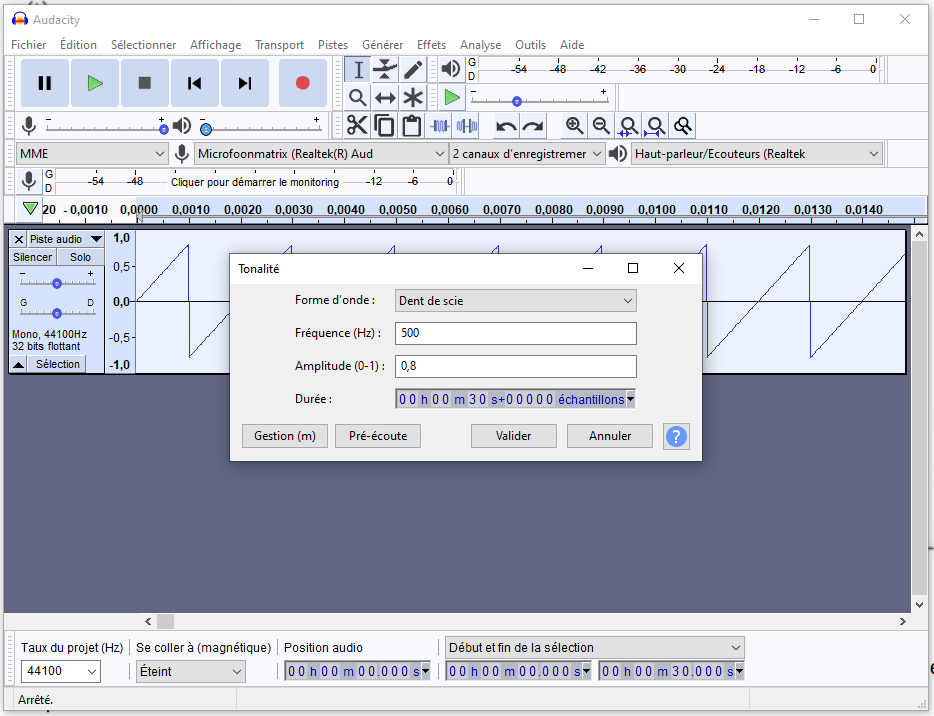
\includegraphics[width=0.85\textwidth]{images/DentScie001.PNG}
    \caption{Génération du signal en dent de scie}
    \label{fig:DentScie001}
\end{figure}

\begin{figure}[H]
    \centering
    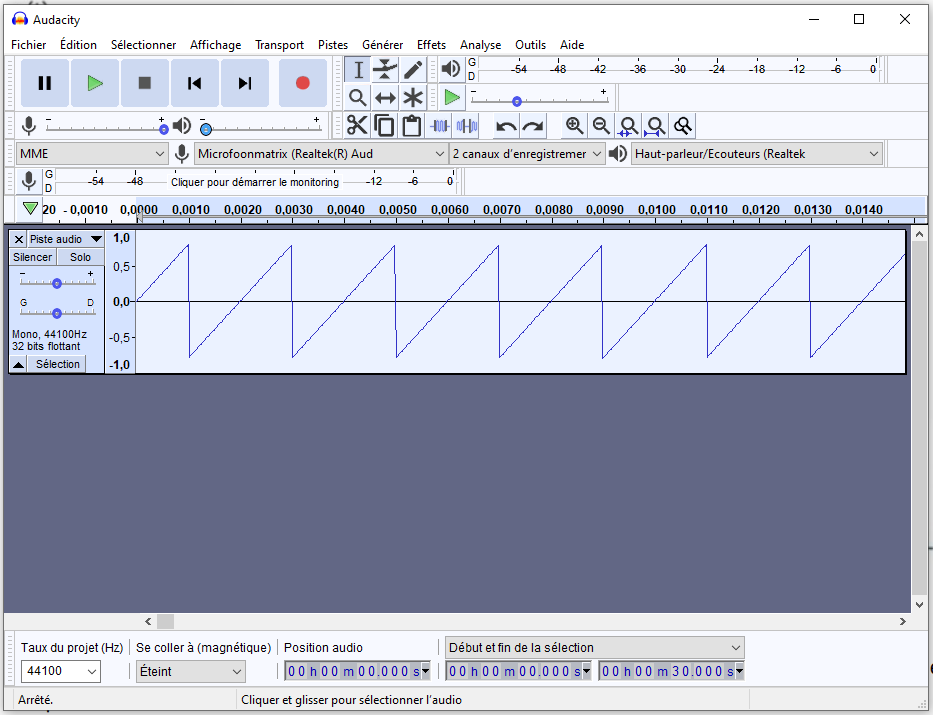
\includegraphics[width=0.85\textwidth]{images/DentScie002.PNG}
    \caption{Représentation temporelle du signal en dent de scie}
    \label{fig:DentScie002}
\end{figure}

\begin{figure}[H]
    \centering
    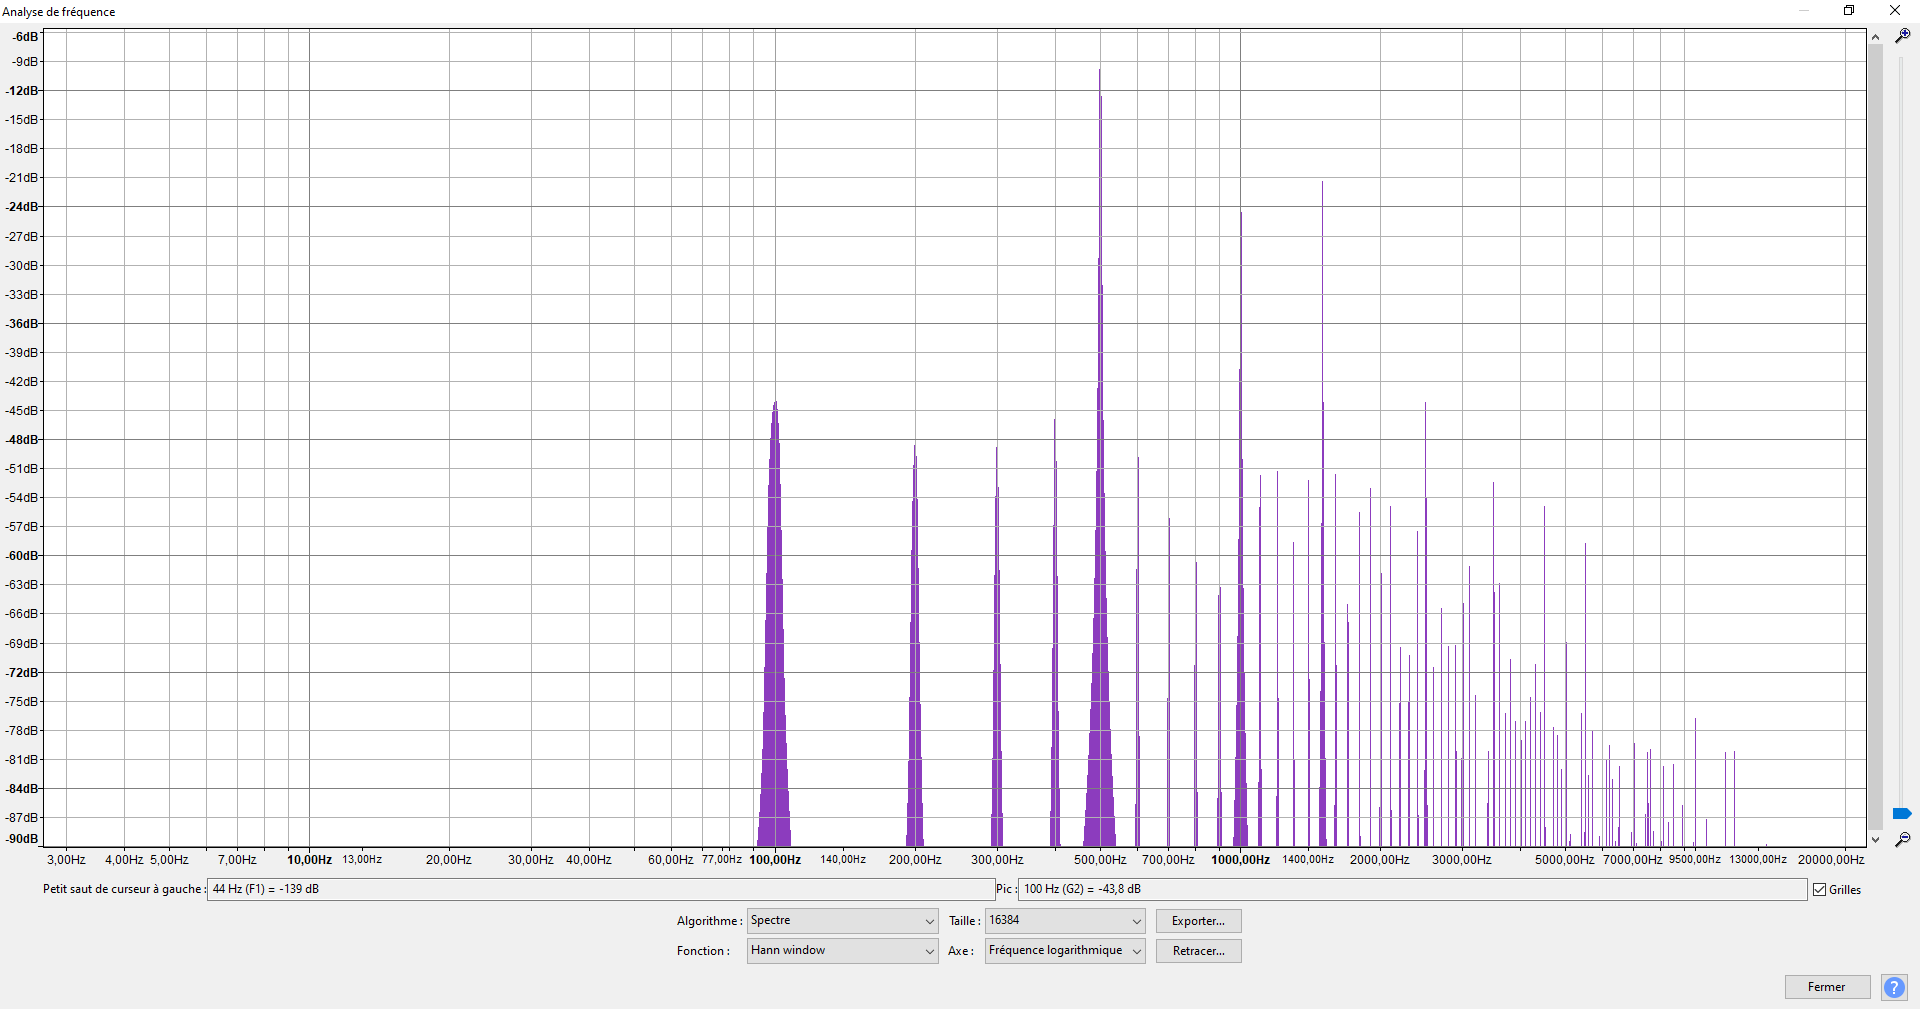
\includegraphics[width=0.85\textwidth]{images/DentScie003.PNG}
    \caption{Représentation spectrale du signal en dent de scie}
    \label{fig:DentScie003}
\end{figure}

%%%%%%%%%%%%%%%%%%%%%%%%%

Nous avons ensuite généré, comme pour l'étude du signal carré, les quatre premières sinusoïdes avant de les mixer avec Audacity et d'observer le résultat sur la figure \ref{fig:DentScie015}. Le problème est que nous avions oublié d'inverser le signal de la seconde et la quatrième sinusoïdes et c'est pour cela que le signal approximé ne ressemble pas au signal en dent de scie.

Nous avons ensuite apporté la correction au sinusoïdes et le signal approximé (figure \ref{fig:DentScie017}) ressemblait désormais au vrai signal en dent de scie créé par Audacity.

%%%%%%%%%%%%%%%%%%%%%%%%%

\begin{figure}[H]
    \centering
    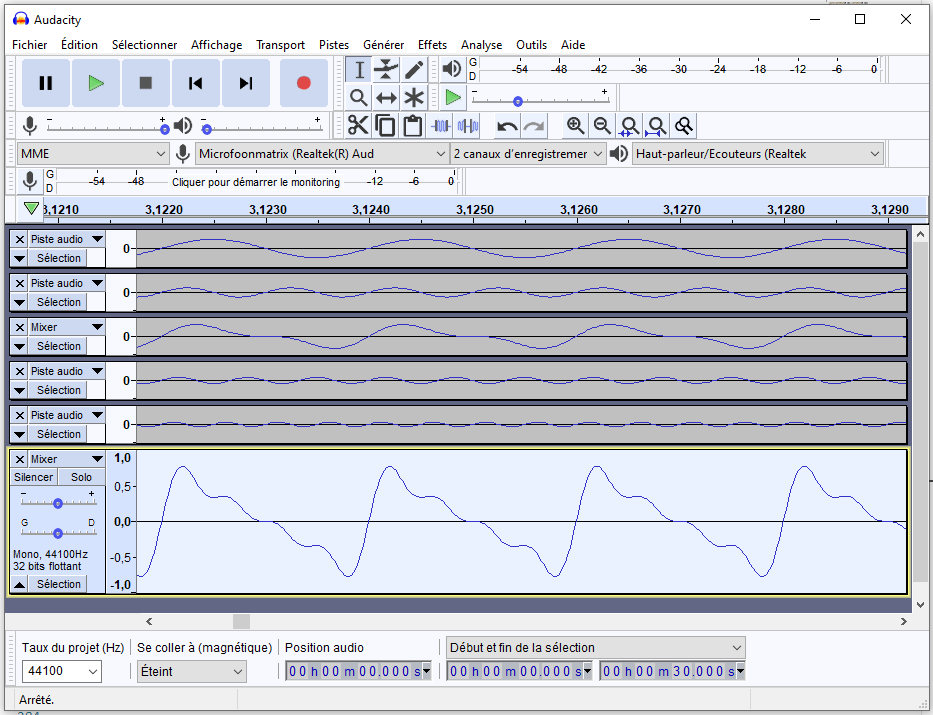
\includegraphics[width=0.85\textwidth]{images/DentScie015.PNG}
    \caption{Mauvaise approximation du signal en dent de scie}
    \label{fig:DentScie015}
\end{figure}

\begin{figure}[H]
    \centering
    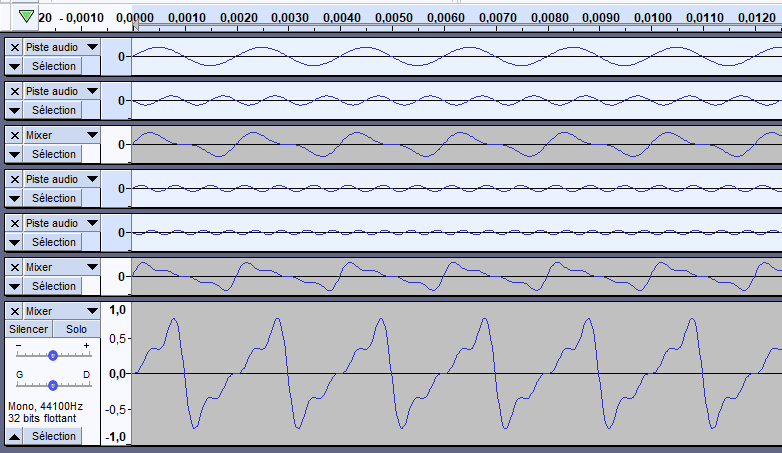
\includegraphics[width=0.85\textwidth]{images/DentScie017.PNG}
    \caption{Bonne approximation du signal en dent de scie}
    \label{fig:DentScie017}
\end{figure}

\begin{figure}[H]
    \centering
    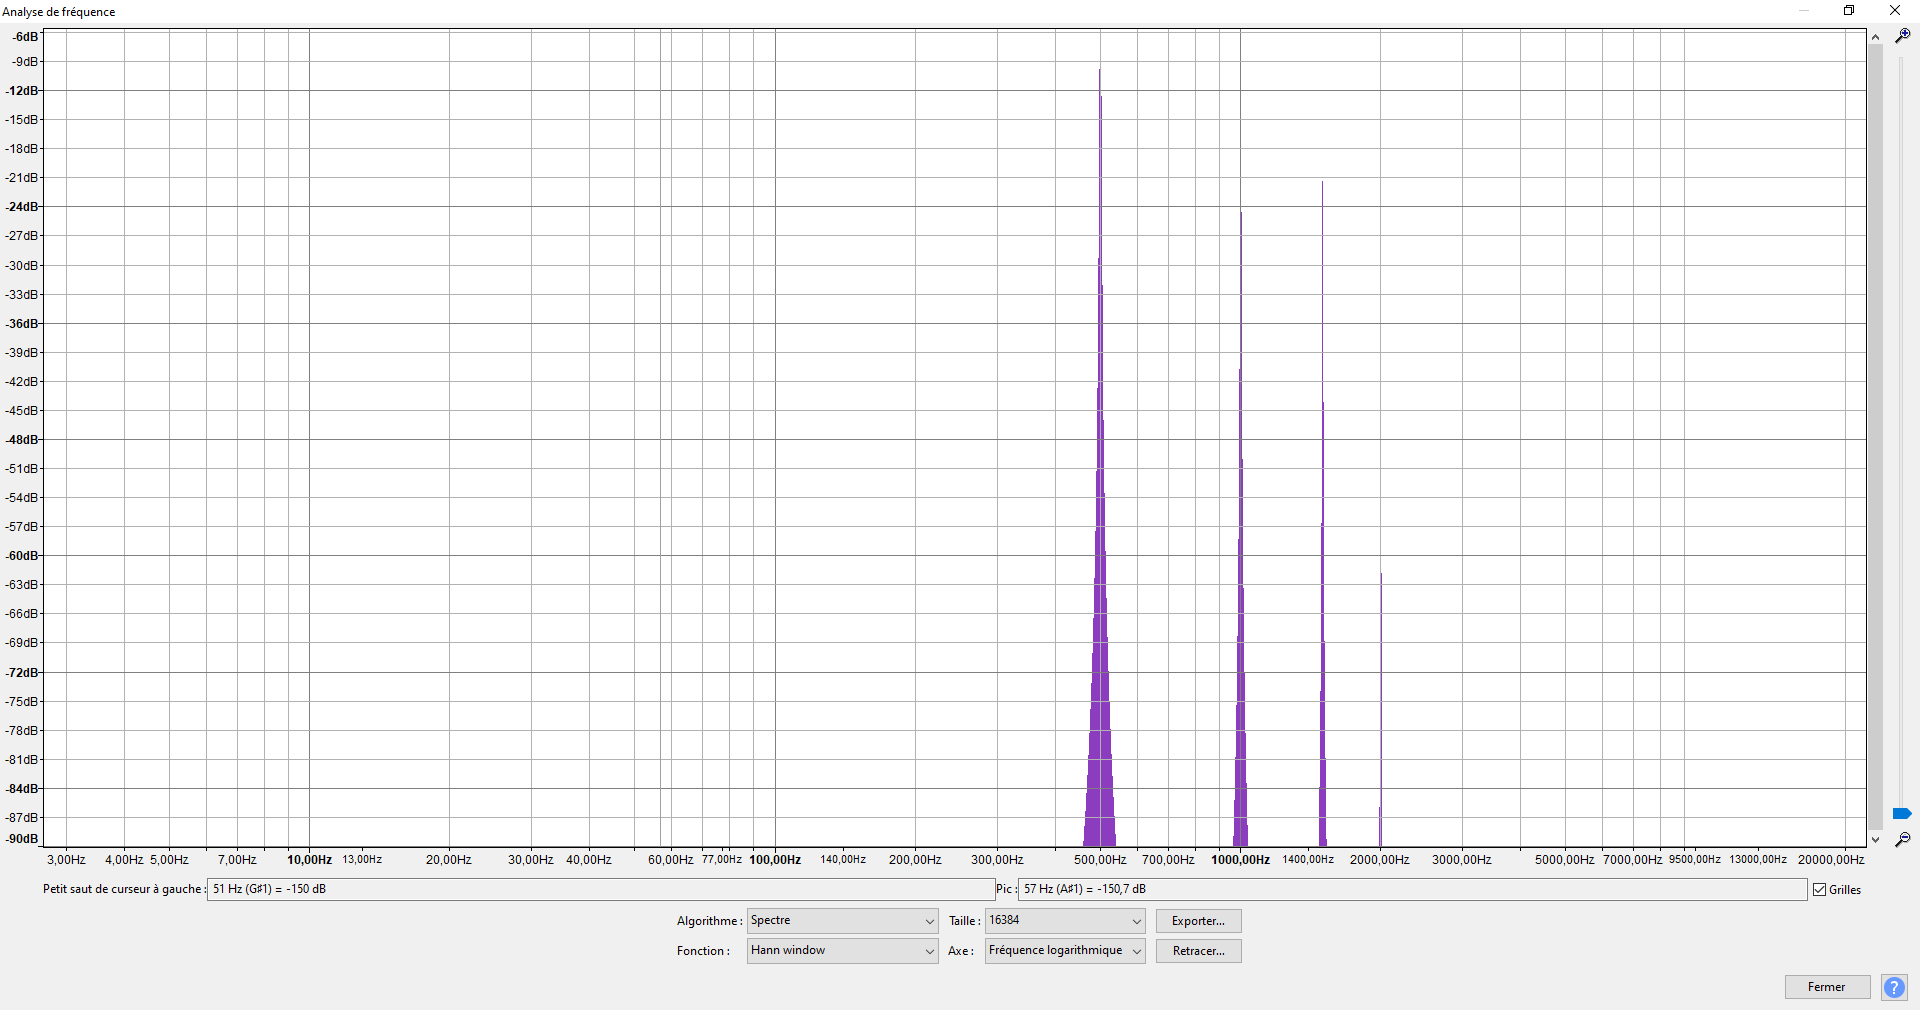
\includegraphics[width=0.85\textwidth]{images/DentScie019.PNG}
    \caption{Représentation spectrale de l'approximation du signal en dent de scie}
    \label{fig:DentScie019}
\end{figure}

%%%%%%%%%%%%%%%%%%%%%%%%%










\subsection{Autre signal}





La série de Fourier de ce signal est donné par la série suivante, qui vient de l'énoncé de la manipulation:
\[ x(t) = \frac{8}{\pi} \bigg( \frac{\sin 2 x \; t}{1 \times 3} - \frac{\sin 4 x \; t}{3 \times 5} + \frac{\sin 6 x \; t}{5 \times 7} - ... \bigg) \]
Les huit premiers signaux que nous devons générer sont donc:
\begin{enumerate}
    \item signal = $\displaystyle +\frac{8}{\pi} \frac{\sin 2 x \; t}{1 \times 3} $, amplitude = 0,849, fréquence = 1000 Hz
    \item signal = $\displaystyle -\frac{8}{\pi} \frac{\sin 4 x \; t}{3 \times 5} $, amplitude = 0,170, fréquence = 2000 Hz
    \item signal = $\displaystyle +\frac{8}{\pi} \frac{\sin 6 x \; t}{5 \times 7} $, amplitude = 0,073, fréquence = 3000 Hz
    \item signal = $\displaystyle -\frac{8}{\pi} \frac{\sin 8 x \; t}{7 \times 9} $, amplitude = 0,040, fréquence = 4000 Hz

    \item signal = $\displaystyle +\frac{8}{\pi} \frac{\sin 10 x \; t}{9 \times 11} $, amplitude = 0,016, fréquence = 5000 Hz
    \item signal = $\displaystyle -\frac{8}{\pi} \frac{\sin 12 x \; t}{11 \times 13} $, amplitude = 0,011, fréquence = 6000 Hz
    \item signal = $\displaystyle +\frac{8}{\pi} \frac{\sin 14 x \; t}{13 \times 15} $, amplitude = 0,008, fréquence = 7000 Hz
    \item signal = $\displaystyle -\frac{8}{\pi} \frac{\sin 16 x \; t}{15 \times 17} $, amplitude = 0,006, fréquence = 8000 Hz
\end{enumerate}
\textbf{Remarque:} puisqu'elle n'était pas donnée, nous avons choisis la fréquence 500 Hz pour ce signal.





%%%%%%%%%%%%%%%%%%%%%%%%%

Pour ce qui est de l'\textit{autre signal}, il était demandé de tester la série de Fourier avec une petite dizaine de signaux sinusoïdaux. Nous avons décidé d'utiliser les huit premiers. Nous avons mixé les sinusoïdes à deux reprises. Une fois avec les quatre premières sinusoïdes (figure \ref{fig:AutreSignal002}) et une fois avec les huit premières (figure \ref{fig:AutreSignal005} et figure \ref{fig:AutreSignal006}). La représentation spectrale du signal est représentée par la figure \ref{fig:AutreSignal007}.

%%%%%%%%%%%%%%%%%%%%%%%%%

\begin{figure}[H]
    \centering
    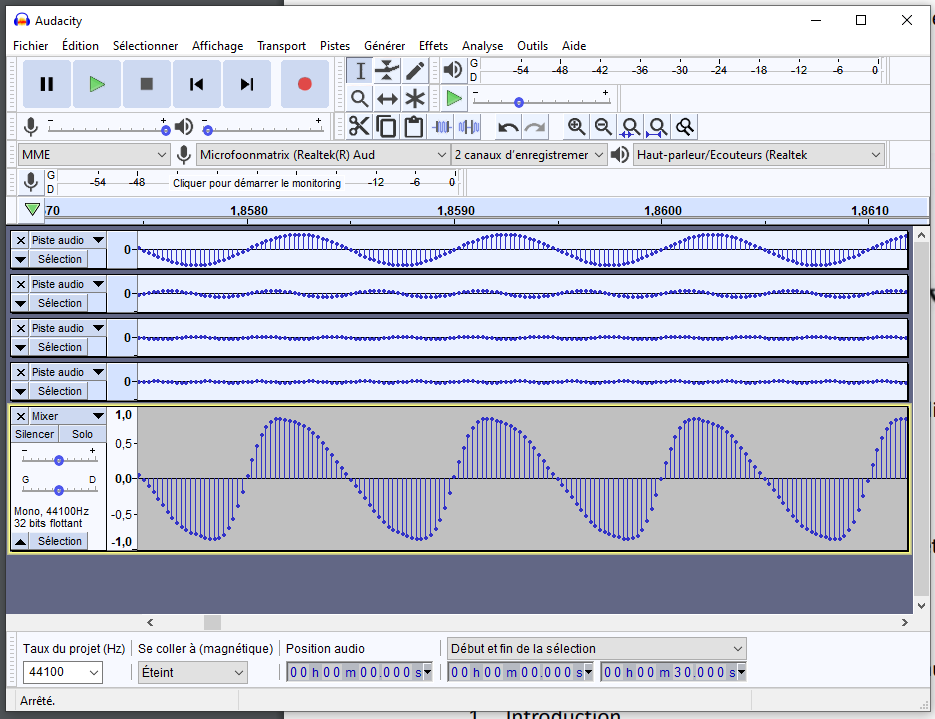
\includegraphics[width=0.85\textwidth]{images/AutreSignal002.PNG}
    \caption{Approximation de l'\textit{autre signal} (4 sinusoïdes)}
    \label{fig:AutreSignal002}
\end{figure}

\begin{figure}[H]
    \centering
    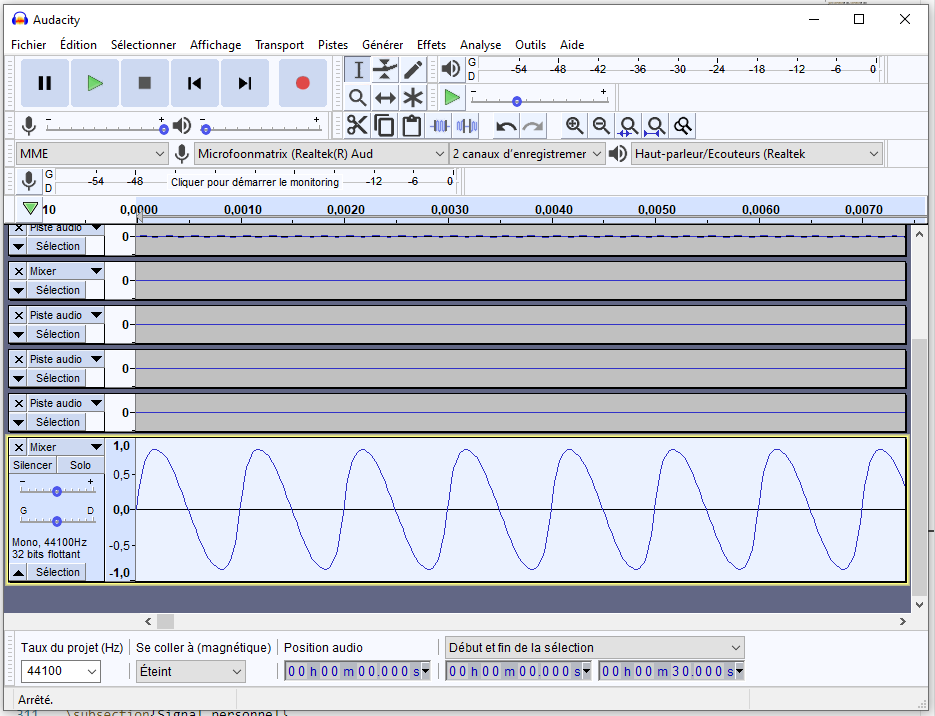
\includegraphics[width=0.85\textwidth]{images/AutreSignal005.PNG}
    \caption{Approximation de l'\textit{autre signal} (8 sinusoïdes)}
    \label{fig:AutreSignal005}
\end{figure}

\begin{figure}[H]
    \centering
    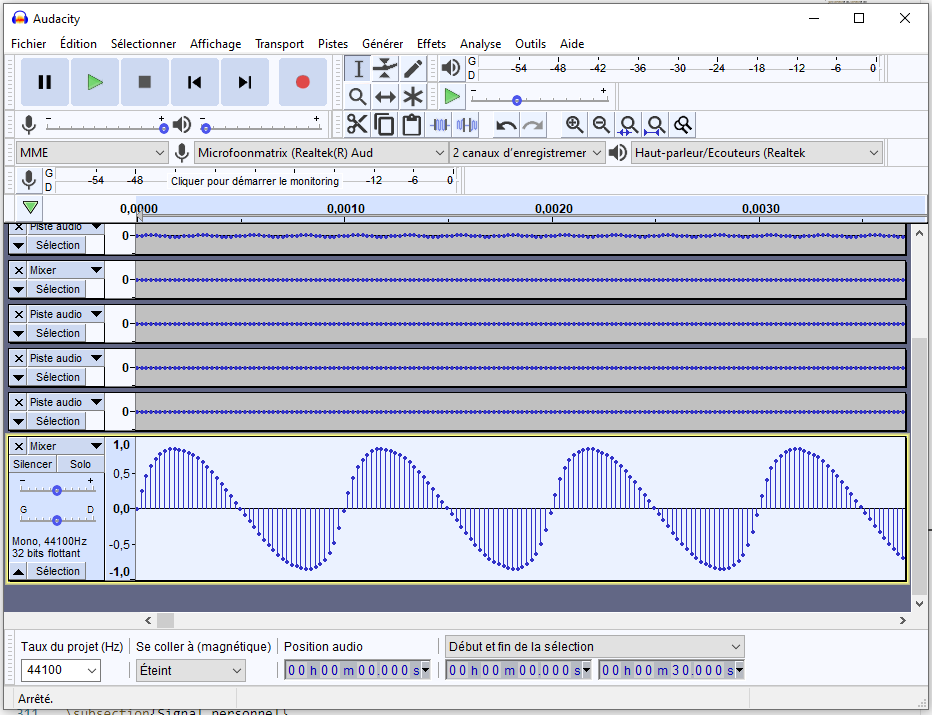
\includegraphics[width=0.85\textwidth]{images/AutreSignal006.PNG}
    \caption{Zoom sur l'approximation de l'\textit{autre signal} (8 sinusoïdes)}
    \label{fig:AutreSignal006}
\end{figure}

\begin{figure}[H]
    \centering
    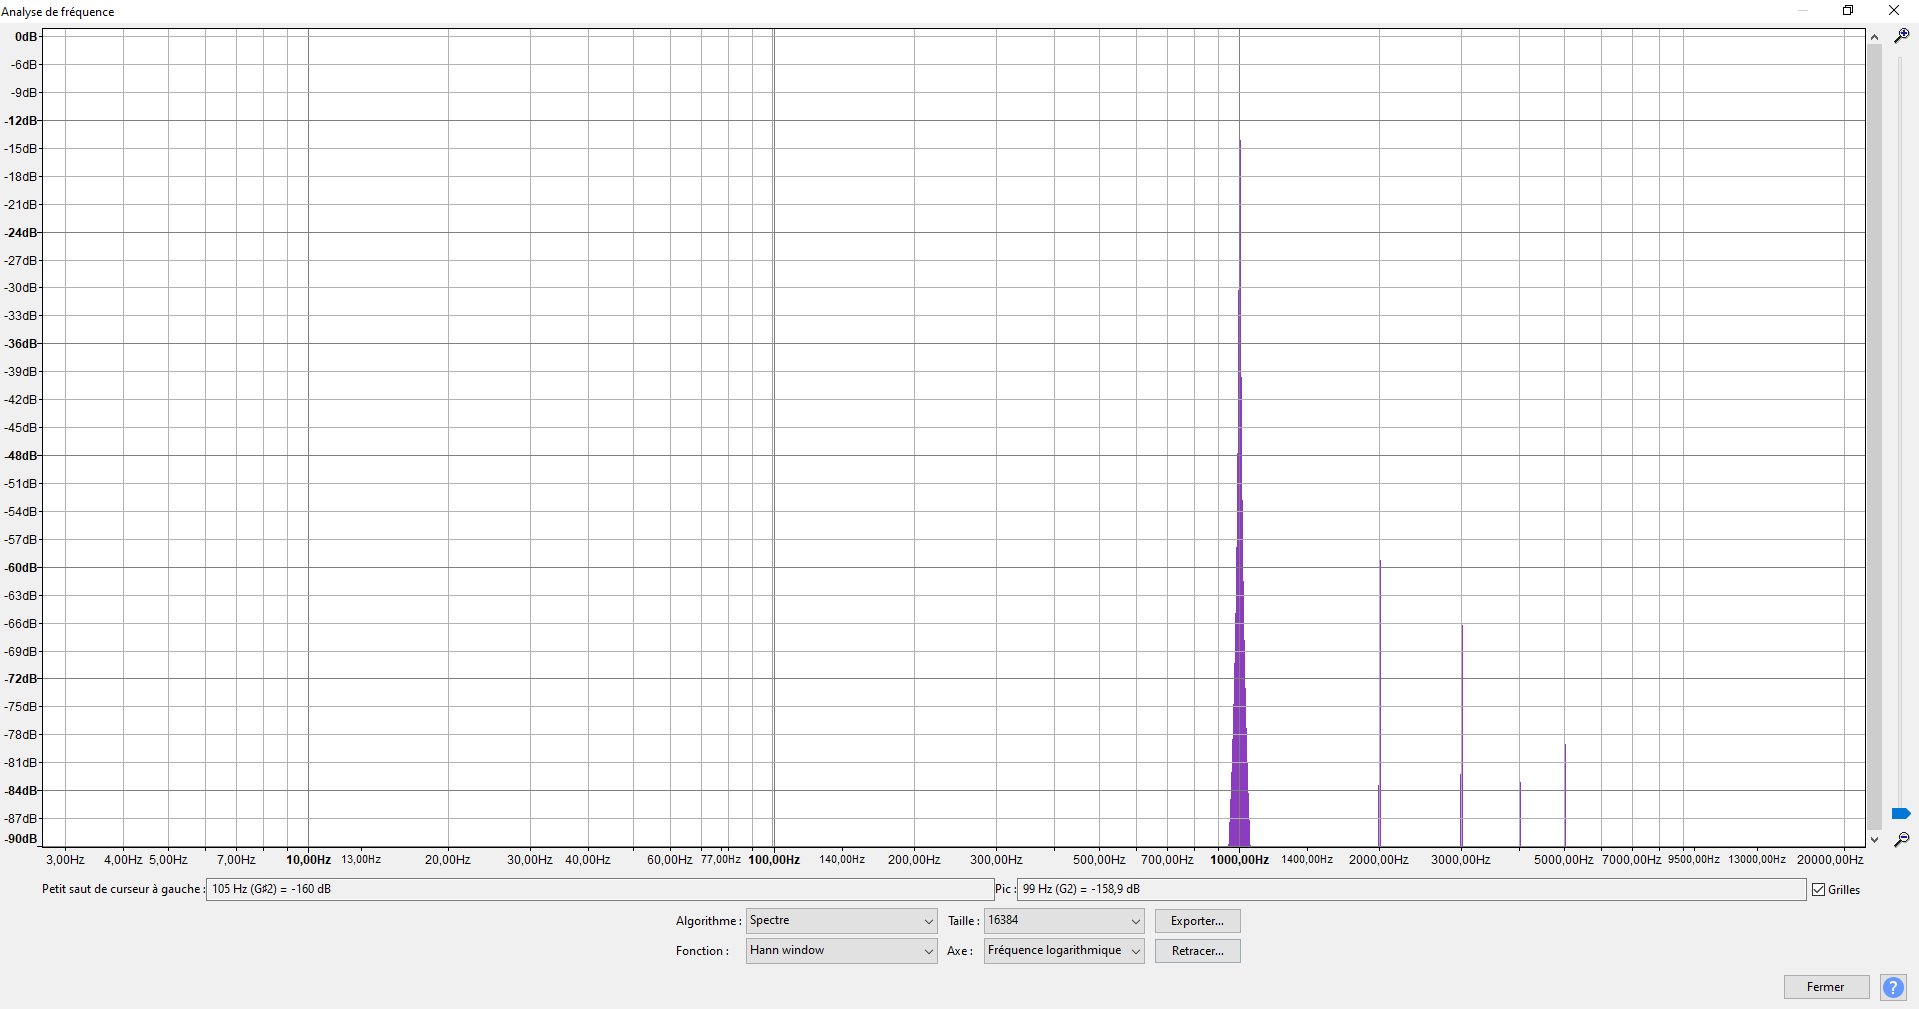
\includegraphics[width=0.85\textwidth]{images/AutreSignal007.PNG}
    \caption{Représentation spectrale de l'approximation de l'\textit{autre signal}}
    \label{fig:AutreSignal007}
\end{figure}

%%%%%%%%%%%%%%%%%%%%%%%%%










\subsection{Signal personnel}





\begin{figure}[H]
    \centering
    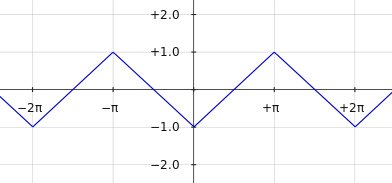
\includegraphics[width=0.75\textwidth]{images/Triangle001.jpg}
    \caption{Signal personnel choisis - signal triangulaire}
    \label{fig:Triangle001}
\end{figure}





Pour notre signal personnel, nous avons pris un signal triangulaire (figure \ref{fig:Triangle001}) qui possède la transformée de Fourier suivante:
\[
    \begin{aligned}
        x(t) &= \frac{8}{\pi^2} \sum_{k=0}^{\infty} (-1)^k \frac{\sin \big( (2 k + 1) \omega t \big)}{(2 k + 1)^2} \\
        &= \frac{8}{\pi^2} \bigg( \sin \omega t - \frac{\sin 3 \omega t}{9} + \frac{\sin 5 \omega t}{25}  - ... \bigg)
    \end{aligned}
\]
Voici les 4 premiers signaux que nous devons générer:
\begin{enumerate}
    \item signal = $\displaystyle + \frac{8}{\pi^2} \frac{\sin 1 \omega t}{1} $, amplitude = 0,810, fréquence = 500 Hz
    \item signal = $\displaystyle - \frac{8}{\pi^2} \frac{\sin 3 \omega t}{9} $, amplitude = 0,090, fréquence = 1500 Hz
    \item signal = $\displaystyle + \frac{8}{\pi^2} \frac{\sin 5 \omega t}{25} $, amplitude = 0,032, fréquence = 2500 Hz
    \item signal = $\displaystyle - \frac{8}{\pi^2} \frac{\sin 7 \omega t}{49} $, amplitude = 0,016, fréquence = 3500 Hz
\end{enumerate}
\textbf{Remarque:} nous avons choisis la fréquence 500 Hz pour ce signal.





%%%%%%%%%%%%%%%%%%%%%%%%%

Pour ce dernier signal, le signal personner, nous avons à nouveau créé quatre sinusoïdes pour les combiner et créer une approximation du signal triangulaire que nous avons choisis. Tout comme pour le signal en dent de scie, nous avions oublié d'inverser certaines sinusoïdes ce qui a donné le cinquième signal sur la figure \ref{fig:SignalPerso001} mais nous l'avons rapidement corrigé pour obtenir le sixième signal de la même figure. La représentation spectrale de ce signal est illustrée par la figure \ref{fig:SignalPerso003}.

%%%%%%%%%%%%%%%%%%%%%%%%%

\begin{figure}[H]
    \centering
    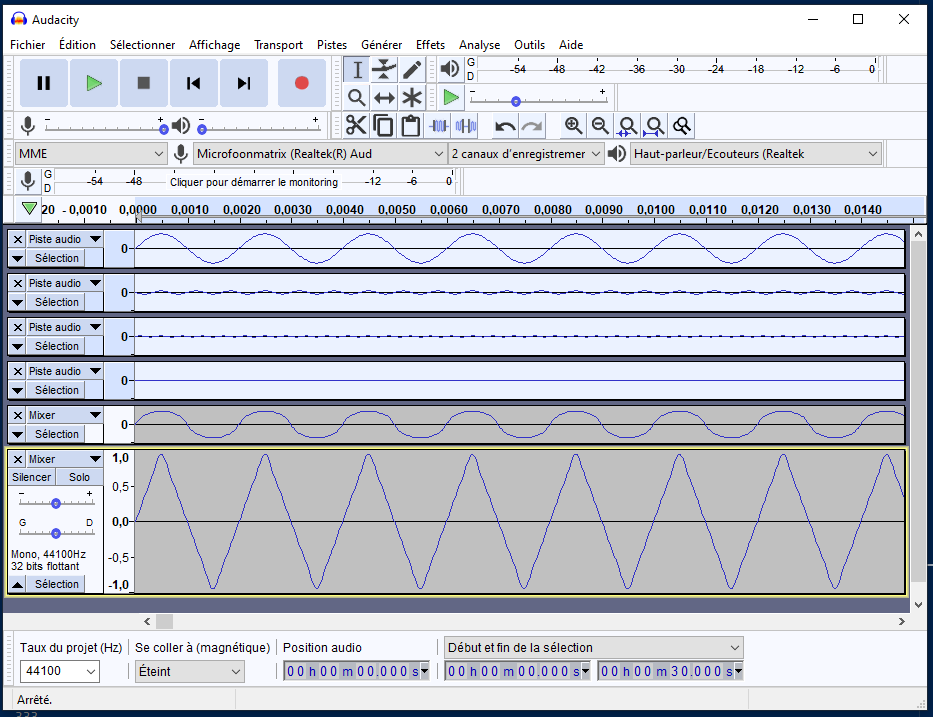
\includegraphics[width=0.75\textwidth]{images/SignalPerso001.PNG}
    \caption{Les quatres sinusoïdes, une mauvaise approximation et une bonne approximation du signal triangulaire}
    \label{fig:SignalPerso001}
\end{figure}

\begin{figure}[H]
    \centering
    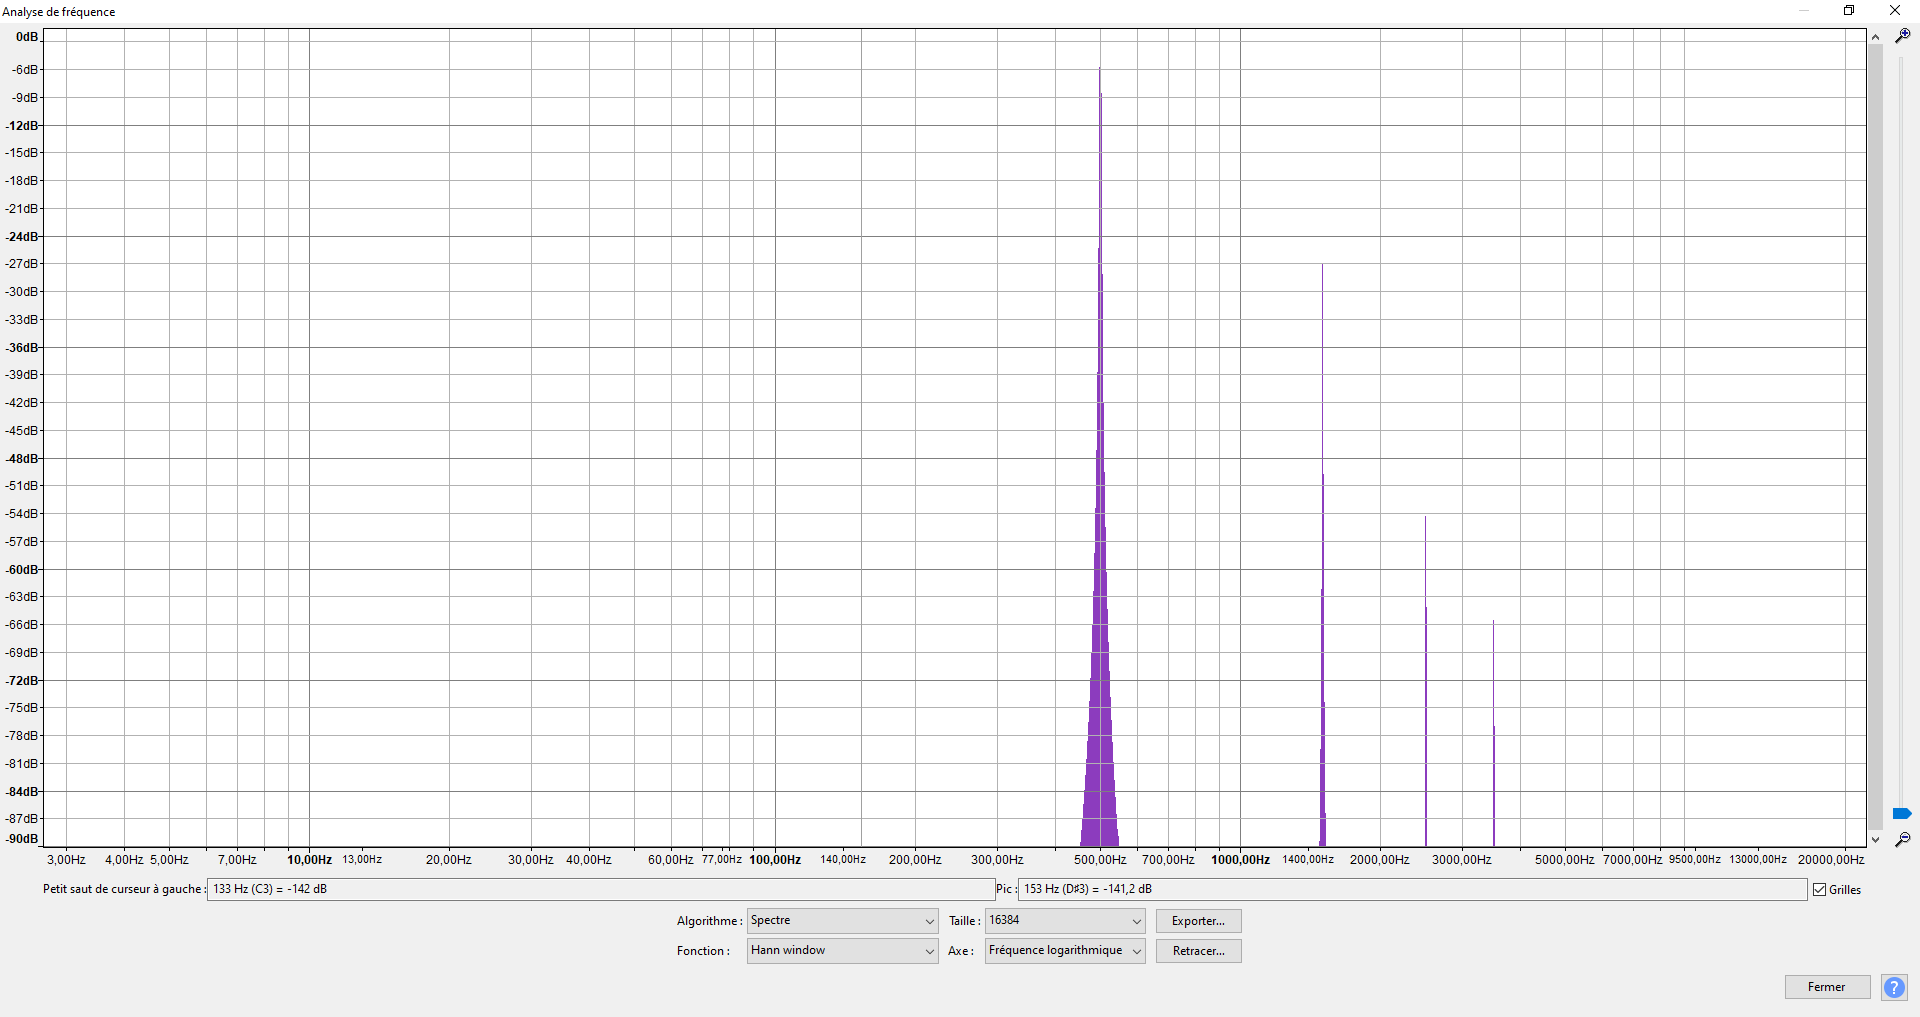
\includegraphics[width=0.75\textwidth]{images/SignalPerso003.PNG}
    \caption{Représentation spectrale de la bonne approximation du signal triangulaire}
    \label{fig:SignalPerso003}
\end{figure}

%%%%%%%%%%%%%%%%%%%%%%%%%















\section{Conclusion}





Pour conclure ce rapport sur la représentation des signaux et l'analyse de Fourier, nous pouvons dire que nous avons appris que la représentation spectrale est tout aussi utile que la représentation temporelle d'un signal périodique et que chaque signal périodique peut être représenté par les sinusoïdes qui le compose. La somme de ces sinusoïdes est une série de Fourier et elle peut servir à approximer des signaux complexes à l'aide de quelques sinusoïdes simples.















\newpage \tableofcontents \listoffigures
\begin{thebibliography}{9}

\bibitem{1} http://www.silicium628.fr/article\_i.php?id=120
\bibitem{2} http://www.cochlea.eu/son/representation-du-son
\bibitem{3} https://fr.wikipedia.org/wiki/Signal\_triangulaire
\bibitem{4} https://fr.wikipedia.org/wiki/S\%C3\%A9rie\_de\_Fourier
\bibitem{5} https://en.wikipedia.org/wiki/Fourier\_series

\end{thebibliography}














\end{document}
